\documentclass[11pt,a4paper,oneside,openany]{scrbook}
\usepackage[palatino]{textbooknotes}
\usepackage{tikz,pgfplots,needspace,float}
\pgfplotsset{compat=1.18}
% Course-local revision layout; retain the shared textbooknotes style unchanged.
\geometry{inner=25mm,outer=30mm,top=20mm,bottom=22mm,
  marginparwidth=18mm,marginparsep=5mm}
\linespread{1.06}
\setlength{\parindent}{0pt}
\setlength{\parskip}{5pt plus 1pt minus 1pt}
\setcounter{tocdepth}{1}
\setkomafont{chapter}{\fontsize{23}{27}\selectfont\bfseries\color{primary}}
\setkomafont{section}{\large\bfseries\color{primary}}
\setkomafont{subsection}{\normalsize\bfseries\color{primary}}
\setkomafont{paragraph}{\normalsize\bfseries\color{primary}}
\renewcommand*{\chapterformat}{\textcolor{accent}{\thechapter}\enskip}
\RedeclareSectionCommand[beforeskip=0pt,afterskip=12pt]{chapter}
\RedeclareSectionCommand[beforeskip=13pt,afterskip=5pt]{section}
\RedeclareSectionCommand[beforeskip=9pt,afterskip=3pt]{subsection}
\RedeclareSectionCommand[runin=false,beforeskip=7pt,afterskip=2pt]{paragraph}
\definecolor{accent}{HTML}{98653C}
\definecolor{defcol}{HTML}{1F4E79}
\definecolor{exacol}{HTML}{287C7A}
\definecolor{remcol}{HTML}{98653C}
\tcbset{tbnbox/.style={enhanced,breakable,sharp corners,boxrule=0pt,
  frame hidden,left=9pt,right=9pt,top=7pt,bottom=7pt,
  colback=#1!4,colbacktitle=#1!4,colframe=#1,coltitle=#1,fonttitle=\bfseries,
  titlerule=0pt,
  borderline west={1.2pt}{0pt}{#1},before skip=8pt,after skip=8pt}}
\setlist{itemsep=3pt,topsep=3pt,parsep=0pt}
\raggedbottom
\widowpenalty=10000
\clubpenalty=10000
% Enable only when building the collected course volume.
\newif\ifcoursevolume
\coursevolumefalse
\newcommand{\summaryauthor}{Eran Rehani}
\title{Physical Models of Biological Systems\\Course 77972}
\subtitle{Lecture summaries}
\author{Notes prepared by \summaryauthor}
\date{2026--2027}
\hypersetup{pdftitle={Physical Models of Biological Systems -- Lecture Summaries},
  pdfauthor={\summaryauthor},pdfsubject={Course 77972, Semester A, 2026--2027}}
\begin{document}
% Course cover: generated cell illustration and two real scientific photographs.
% Image provenance and reuse terms: Lecture_Summaries/cover_image_sources.md.
\begin{titlepage}
\thispagestyle{empty}
\begin{tikzpicture}[remember picture,overlay]
\fill[primary!2] (current page.south west) rectangle (current page.north east);
\fill[primary] (current page.north west)
  rectangle ([yshift=-186mm]current page.north east);
\fill[exacol] ([yshift=-186mm]current page.north west)
  rectangle ([yshift=-188mm]current page.north east);
\node[anchor=north west,text=white!80,font=\small\sffamily,
  text width=155mm,align=left]
  at ([xshift=25mm,yshift=-21mm]current page.north west)
  {THE HEBREW UNIVERSITY OF JERUSALEM\\[3pt]Racah Institute of Physics};
\node[anchor=north west,text=white,font=\small\sffamily\bfseries]
  at ([xshift=25mm,yshift=-41mm]current page.north west)
  {COURSE 77972};
\node[anchor=north west,text=white,text width=160mm,align=left,
  font=\fontsize{29}{35}\selectfont\bfseries]
  at ([xshift=25mm,yshift=-54mm]current page.north west)
  {Physical Models of\\Biological Systems};
\node[anchor=north west,text=white!85,font=\large]
  at ([xshift=25mm,yshift=-91mm]current page.north west)
  {Lecture summaries \enspace\textbullet\enspace Exam revision};
% Native 1024 x 1536 illustration: 55 mm tall gives approximately 709 ppi.
\node[inner sep=0pt] at ([xshift=50mm,yshift=-140mm]current page.north west)
  {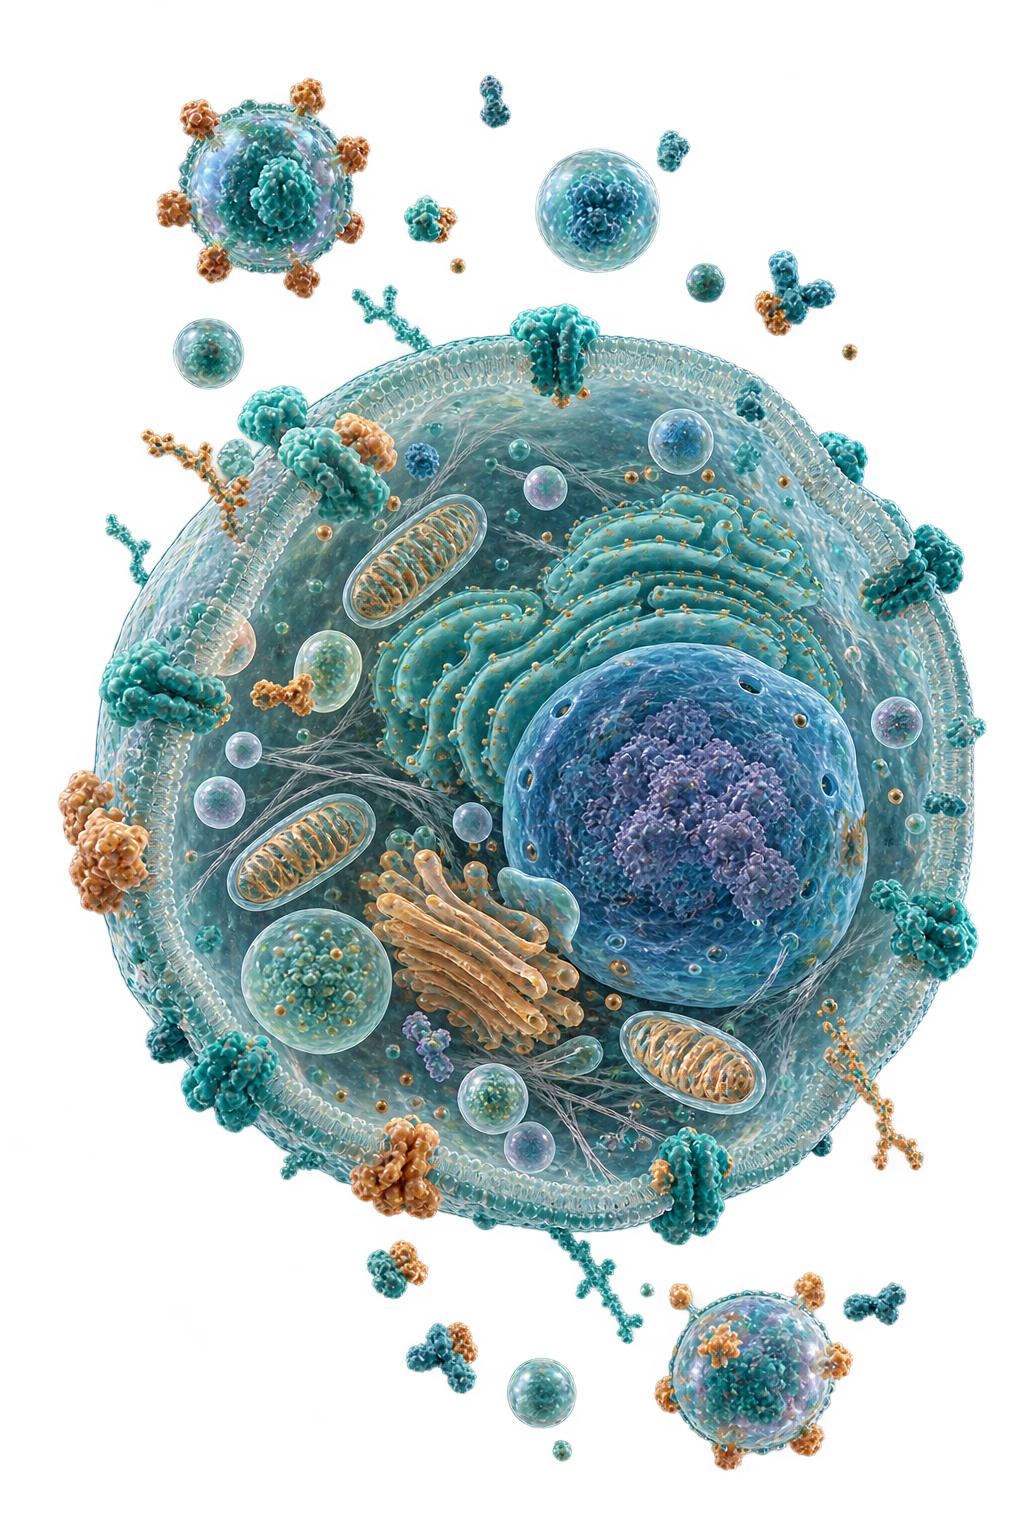
\includegraphics[height=55mm]{Lecture_Summaries/cover_biological_systems.png}};
% Original branching-colony photograph supplied by the user; no recoloring.
\node[inner sep=0pt] at ([xshift=105mm,yshift=-140mm]current page.north west)
  {\includegraphics[width=50mm]{Lecture_Summaries/cover_branching_colony.jpg}};
% Layout-only square crop of the original NOAA photograph; no recoloring.
\begin{scope}
\clip ([xshift=135mm,yshift=-115mm]current page.north west)
  rectangle ([xshift=185mm,yshift=-165mm]current page.north west);
\node[inner sep=0pt] at ([xshift=160mm,yshift=-140mm]current page.north west)
  {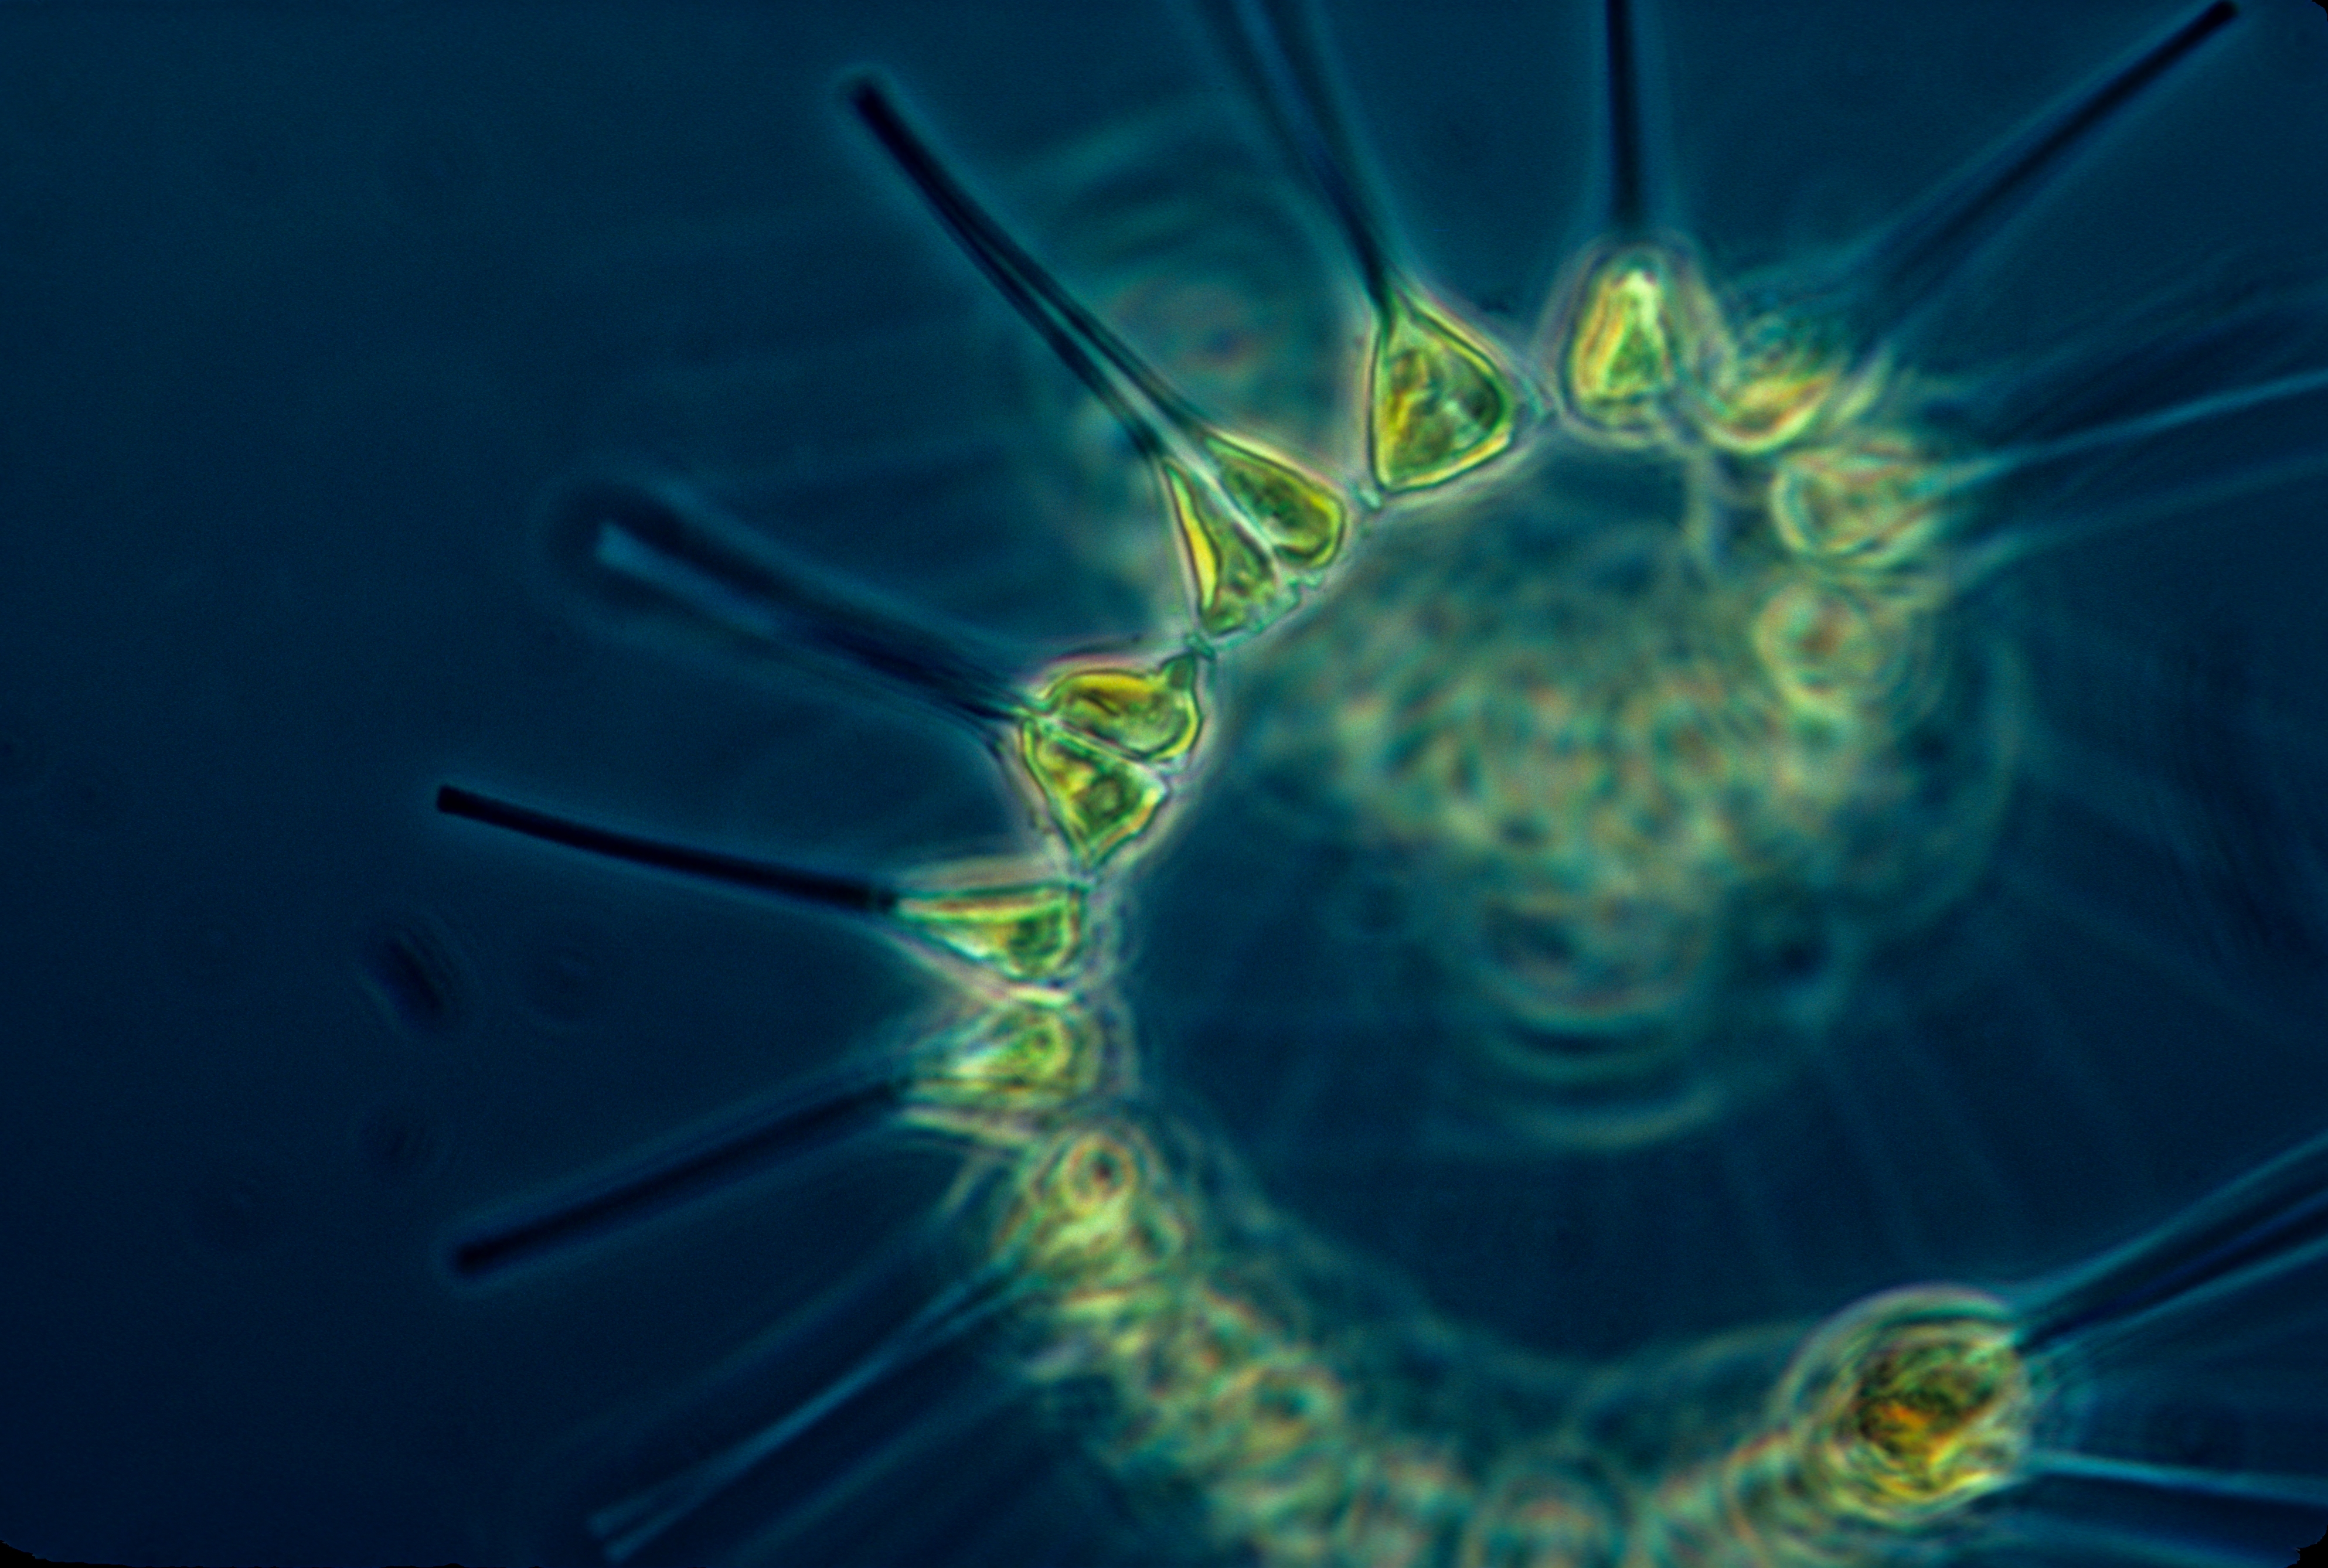
\includegraphics[height=50mm]{Lecture_Summaries/cover_plankton.jpg}};
\end{scope}
\foreach \x/\caption in {50/Cellular mechanisms,105/Microbial populations,160/Phytoplankton}
  \node[text=white!85,font=\small\sffamily]
    at ([xshift=\x mm,yshift=-175mm]current page.north west) {\caption};
\node[anchor=north west,text=primary,font=\large\bfseries]
  at ([xshift=25mm,yshift=-200mm]current page.north west)
  {2026--2027 \enspace|\enspace Semester A};
\node[anchor=north west,text=primary!85!black,align=left,
  font=\normalsize,inner sep=0pt]
  at ([xshift=25mm,yshift=-218mm]current page.north west)
  {\begin{tabular}{@{}ll@{}}
    \textbf{Lecturer} & Dr. Amir Erez\\[8pt]
    \textbf{Notes prepared by} & \summaryauthor
  \end{tabular}};
\node[anchor=north west,text=primary!80!black,font=\scriptsize,
  text width=155mm,align=left,inner sep=0pt]
  at ([xshift=25mm,yshift=-257mm]current page.north west)
  {Cover: AI-generated conceptual cell illustration; branching colony:
   \href{https://commons.wikimedia.org/wiki/File:Microscope_view_of_a_branched_Bacillus_bacterial_colony_08.jpg}{Korinna (2020)},
   \href{https://creativecommons.org/licenses/by/4.0/}{CC BY 4.0};
   phytoplankton: NOAA MESA Project, NOAA Photo Library, public domain, cropped.};
\draw[primary!25,line width=0.5pt]
  ([xshift=25mm,yshift=19mm]current page.south west)--
  ([xshift=-25mm,yshift=19mm]current page.south east);
\node[anchor=south west,text=primary!75,font=\small,text width=155mm]
  at ([xshift=25mm,yshift=10mm]current page.south west)
  {Personal revision notes based on lectures and course materials.};
\end{tikzpicture}
\null
\end{titlepage}

\ifcoursevolume
  \tableofcontents
\fi
\pagenumbering{arabic}
\setcounter{chapter}{-1}
% Course: 77972 -- Physical Models of Biological Systems
% Academic year: 2026--2027 | Semester: A
% Lecture number: 1 | Document chapter: 0 (course introduction)
% Lecture date: 2026-10-13
% Title: Introduction
% Lecturer: Dr. Amir Erez
% Notes prepared by: Eran Rehani
% Source: Lecture Transcripts/77972_2026-10-13_שעור_א_Captions_עברית_Hebrew.md
% Main conceptual discussion: 00:10:48--00:37:06; modelling cycle: 00:48:54--00:49:18.
% Supporting references: models-notes-2026.pdf, chapter 0, printed pp. 9--11;
% Philip Nelson, Physical Models of Living Systems, chapter 2.
\chapter{Introduction}\label{chap:introduction}
\noindent\textbf{From Lecture 1 \enspace|\enspace 13 October 2026}

Physical modelling connects biological mechanisms to observations. A useful model makes a question precise enough to calculate and test, with explicit assumptions and limitations.

\section{Why living systems need selective descriptions}\label{sec:intro-complexity}
Living systems interact, adapt, and alter their surroundings: photosynthesis changed the atmosphere and hence the conditions for later life.

They maintain organization by exchanging matter and energy with their surroundings. This respects the second law: a steady biological state need not be thermodynamic equilibrium.

\section{What a mathematical model contributes}\label{sec:intro-model-purpose}
A model specifies \textbf{variables}, \textbf{processes}, and their \textbf{relations}, then derives consequences not already inserted by hand.
\begin{itemize}
\item \textbf{Consistency:} equations make a verbal explanation precise and resolve competing effects quantitatively.
\item \textbf{Prediction:} unexpected observations expose missing processes or faulty assumptions; precise biological forecasts remain difficult.
\item \textbf{Inference:} observations constrain hidden rates or interactions when direct measurement is difficult or perturbs the living system.
\item \textbf{Intuition:} a simple model isolates the dominant mechanism and helps us anticipate responses to change.
\end{itemize}

\section{Choose the scale, then test the assumptions}\label{sec:intro-description}
Choose among molecules, cells, populations, communities, and ecosystems. Do space, fluctuations, or discrete individuals matter? Retain the relevant mechanism; add detail when it changes the conclusion.

Data and mechanisms complement each other. Ice-cream searches reveal annual periodicity without modelling its cause: predictive correlation need not explain a mechanism.

\textbf{The modelling cycle:} formulate $\to$ solve $\to$ compare with data $\to$ revise. Agreement supports usefulness, rather than proving every assumption. Chapter~\ref{chap:lecture01} applies this cycle to hidden viral turnover.

\subsection*{How to use these notes for revision}
State assumptions, explain each equation term, and interpret results biologically. Attempt analytical homework before consulting solutions; these problems prepare you for the test. Vary simulation parameters to build intuition.

\subsection*{Further Reading}
\begingroup\small
Amir Erez, course notes, Chapter~0, pp.~9--11; Philip Nelson, \emph{Physical Models of Living Systems}, Chapter~2, ``Physics and Biology.''
\endgroup

% Source transcript: Lecture Transcripts/77972_2026-10-13_שעור_א_Captions_עברית_Hebrew.md
% Course conventions and mathematical cross-check: models-notes-2026.pdf, chapters 0--1, pp. 9--18.
% The supplied transcript is auto-generated Hebrew and contains speech-recognition errors.

\chapter{Modelling Living Systems: Hidden HIV Turnover}\label{chap:lecture01}

\section{Why model living systems?}\label{sec:why-model}

Living systems contain many interacting parts, respond to changing surroundings, and can change those surroundings in turn. A model makes one biological question manageable by naming the relevant variables and processes, stating how they are related, and deriving consequences. It is useful when those consequences teach us something beyond what we put into the assumptions.

\subsection{What mathematics adds}\label{subsec:model-goals}

The lecture described four connected reasons to model biological systems (00:15:54--00:30:48).

\begin{enumerate}
    \item \textbf{Consistency.} A verbal story can leave two competing effects unresolved. Equations make assumptions explicit and determine the combined result.
    \item \textbf{Prediction.} A model can forecast how a system will respond under new conditions. Because every biological model leaves out detail, disagreement with an observation tells us to examine the assumptions and scope.
    \item \textbf{Inference.} Many quantities of interest, such as production and clearance rates, cannot be measured directly. A model can connect them to observable data.
    \item \textbf{Intuition.} A simple model can make the dominant mechanism clear enough to anticipate what should happen when conditions change.
\end{enumerate}

Mechanistic models and data-driven approaches answer related but different questions. A statistical model can predict a pattern without identifying its cause. For example, ice-cream searches and seasonal changes may rise and fall together because both respond to the season; their correlation alone does not show that one causes the other. A mechanistic account proposes a causal chain that can be tested. The two approaches can complement one another: patterns suggest hypotheses, and mechanisms help assess them.

\subsection{Choose the level of description}\label{subsec:description-level}

Questions can concern molecular shape, the behaviour of individual cells, population abundance, interactions between communities, or whole ecosystems. At each level, a modeller chooses which details matter. For example: should we follow individual cells or use a cell density? Are fluctuations important, or is an average adequate? Must space be represented? Are the relevant quantities discrete counts or continuous concentrations?

A sensible starting point is the simplest model that could answer the stated question. It should be refined when observations or the question require more detail. A model that omits the process responsible for the phenomenon is too simple; adding detail that changes no conclusion only makes it harder to understand.

Living systems exchange matter and energy with their surroundings. They can maintain organized structures while those fluxes continue. A steady biological state is therefore a balance of dynamical processes, not necessarily thermodynamic equilibrium. This does not imply a violation of the second law: the system is open and dissipates energy.

\subsection{The modelling cycle}\label{subsec:modelling-cycle}

The recurring procedure is to formulate a question and model, solve the model, compare its consequences with data, and revise the model when needed (00:48:54--00:49:18). Validation asks whether the model is useful for its particular purpose; it does not establish that every biological detail has been represented.

\section{A steady viral load can hide rapid turnover}\label{sec:steady-turnover}

\subsection{The biological puzzle}\label{subsec:hiv-puzzle}

The lecture introduced the HIV viral-load trajectory as a puzzle (00:49:24--00:53:24). In the untreated schematic, viral abundance first rises during an acute stage, falls to a comparatively low plateau that may persist for years, and rises again as disease progresses. The time axis is schematic, and these stages should not be read as a present-day prognosis. A nearly constant viral load does not by itself show that virus production has stopped or become slow.

One possible story is that the virus becomes mostly inactive during the plateau. A different possibility is that production and clearance are both rapid and nearly balanced. The distinction matters because the same steady measurement is compatible with very different underlying fluxes.

\subsection{A leaky container and a stable state}\label{subsec:container}

Consider a container with liquid volume $W(t)$. Liquid enters at volumetric rate $Q_{\mathrm{in}}$ and leaves at rate $Q_{\mathrm{out}}$. Conservation of volume gives
\begin{equation}\label{eq:container-balance}
    \frac{\dd W}{\dd t}=Q_{\mathrm{in}}-Q_{\mathrm{out}}.
\end{equation}
Here $W$ has units of volume and both flow rates have units of volume per time. At a steady volume,
\begin{equation}\label{eq:container-steady}
    Q_{\mathrm{in}}=Q_{\mathrm{out}}.
\end{equation}
This equality tells us that the two flows match; it does not tell us whether either one is small or large. A calm-looking water level can conceal rapid replacement of its contents. The same reasoning applies to a population or concentration maintained by balanced production and removal.

Why can outflow rise with the amount of liquid? For a liquid column with constant cross-sectional area $A$ and height $h$, force balance between its bottom and top gives
\begin{equation}\label{eq:hydrostatic-balance}
    p_{\mathrm{bottom}} A=p_{\mathrm{top}} A+mg,
\end{equation}
where $p_{\mathrm{bottom}}$ and $p_{\mathrm{top}}$ are pressures, $m$ is the liquid mass, and $g$ is gravitational acceleration. Since $m=\rho A h$, with mass density $\rho$, division by $A$ yields
\begin{equation}\label{eq:hydrostatic-pressure}
    p_{\mathrm{bottom}}-p_{\mathrm{top}}=\rho g h.
\end{equation}
For the viscous outlet considered in the lecture, Poiseuille flow makes the outflow proportional to this pressure difference. Therefore $Q_{\mathrm{out}}\propto h$. Because $W=Ah$ for fixed $A$, the outflow is also proportional to the stored volume. This proportionality depends on the flow regime and outlet; it is not a universal rule for every hole or container.

As a simple mathematical version of this mechanism, let $Q_{\mathrm{out}}=\kappa W$, where $\kappa>0$ has units of inverse time. Then
\begin{equation}\label{eq:container-dynamics}
    \frac{\dd W}{\dd t}=Q_{\mathrm{in}}-\kappa W.
\end{equation}
At steady state, $W^*=Q_{\mathrm{in}}/\kappa$. If $\delta W=W-W^*$ is a small deviation, subtract the steady-state equation from the dynamical equation to obtain
\begin{equation}\label{eq:container-perturbation}
    \frac{\dd\,\delta W}{\dd t}=-\kappa\delta W,
    \qquad \delta W(t)=\delta W(0)\ee^{-\kappa t}.
\end{equation}
An excess volume drains away, while a deficit reduces outflow and allows the constant input to refill the container. Thus the balance is stable in this simple model.

\begin{example}{Worked Example: A leaky container}{container-example}
Suppose water enters at $Q_{\mathrm{in}}=2\,\mathrm{mL/min}$, and the outlet law is $Q_{\mathrm{out}}=0.1\,W\,\mathrm{min}^{-1}$ when $W$ is measured in millilitres. The steady volume solves $0=2\,\mathrm{mL/min}-0.1\,\mathrm{min}^{-1}W^*$, so $W^*=20\,\mathrm{mL}$. If the container is at $25\,\mathrm{mL}$, the instantaneous net change is $2-0.1(25)=-0.5\,\mathrm{mL/min}$; the volume falls toward $20\,\mathrm{mL}$. If it is at $15\,\mathrm{mL}$, the net change is $+0.5\,\mathrm{mL/min}$ and the volume rises toward the same steady value.

\textit{Significance:} The steady amount is set by the ratio of input to clearance, so observing that amount alone does not reveal the turnover speed.
\end{example}

The HIV hypothesis is that viral production and clearance can both be large during the plateau. The container analogy explains the possibility; a time-dependent perturbation is needed to estimate the hidden rates.

\section{Perturbing HIV reveals hidden rates}\label{sec:hiv-perturbation}

\subsection{Treatment as a probe}\label{subsec:treatment-probe}

The lecture discussed a 1994 study in which antiviral treatment was followed by a rapid decline in measured viral RNA (01:04:48--01:06:54). The initial load was of order $10^5$ RNA copies per millilitre, and the early decline was roughly two orders of magnitude over about a week to ten days. On a semilogarithmic plot, an exponential decline appears approximately as a straight line. The observed initial plateau and subsequent decline indicate that the curve is not one exponential over its full time course.

The treatment discussed inhibits HIV protease, an enzyme that cleaves a viral polyprotein into functional parts. Inhibiting this processing reduces the production of mature, infectious virions. It does not instantly stop already infected cells from releasing viral material. This distinction motivates the model below: treatment blocks new cell infections, while previously infected cells continue to produce virions until they are cleared.

HIV is a retrovirus: its RNA is copied into DNA by reverse transcription. Copying errors generate variants, and natural selection changes their abundances when conditions favour one variant. In a simplified independent-mutation model, if resistance to each of $n$ drugs requires a distinct mutation with probability $p$, then the probability of acquiring all required mutations in one replication opportunity is $p^n$. This is a mathematical illustration of why independent barriers can help; it assumes no cross-resistance and does not prescribe a clinical regimen.

\begin{example}{Worked Example: Independent resistance barriers}{resistance-example}
Suppose there are $M=10^9$ replication opportunities in a chosen interval, and each of three distinct resistance mutations has probability $p=10^{-5}$ per opportunity. The expected number of single-drug-resistant mutants is $Mp=10^4$. Under the much stronger assumption that all three mutations must arise together in one opportunity and are independent, the expected number of triple-resistant mutants in that interval is $Mp^3=10^9(10^{-5})^3=10^{-6}$. The calculation is an expectation under a toy model, not a prediction of the probability that resistance already exists: it omits mutation histories, selection, population structure, and correlated resistance.

\textit{Significance:} Independence makes simultaneous barriers multiply in probability, but the assumptions determine whether that multiplication applies.
\end{example}

\subsection{The post-treatment variables and assumptions}\label{subsec:hiv-variables}

For times $t\geq0$, let $N_I(t)$ be the number of infected cells and $N_V(t)$ the number of free virions in a chosen compartment. The measured assay is often reported as RNA copies per millilitre; to use absolute counts instead, one must specify the compartment volume. Either convention works if production and clearance terms use consistent units. We use $N_I(0)=N_{I0}$ and $N_V(0)=N_{V0}$.

The model assumes that treatment at $t=0$ completely blocks new infections; infected cells already present remain able to produce virions. Each infected cell is cleared with constant per-cell rate $k_I$, and each free virion with constant rate $k_V$. Both rate constants have units of inverse time. Each infected cell produces virions at rate $\gamma$ (virions per cell per unit time), and we define $\beta=\gamma N_{I0}$, the initial production rate. This minimal model treats the measured compartment as well mixed over the time window and omits cell-to-cell variation and long-lived latent reservoirs.

Before treatment, the viral load is assumed to be approximately steady. Its production and free-virion clearance balance:
\begin{equation}\label{eq:hiv-presteady}
    \gamma N_{I0}=k_VN_{V0},
    \qquad \beta=k_VN_{V0}.
\end{equation}
This is an initial condition supplied by the pre-treatment state, not an extra post-treatment process.

\subsection{Derive the infected-cell dynamics}\label{subsec:infected-cells}

If an individual infected cell has a constant clearance probability per unit time $k_I$, then in a short time $\Delta t$ its probability of clearance is $k_I\Delta t+o(\Delta t)$. Among $N_I$ cells, the expected number lost in that interval is $k_I N_I\Delta t$ to leading order. Dividing the change $\Delta N_I=-k_I N_I\Delta t$ by $\Delta t$ and taking the limit gives
\begin{equation}\label{eq:infected-ode}
    \frac{\dd N_I}{\dd t}=-k_IN_I.
\end{equation}
Separate variables and integrate from $0$ to $t$:
\begin{equation}\label{eq:infected-integral}
    \int_{N_{I0}}^{N_I(t)}\frac{\dd N_I}{N_I}
    =-k_I\int_0^t\dd s,
    \qquad \ln\!\left(\frac{N_I(t)}{N_{I0}}\right)=-k_It.
\end{equation}
Exponentiating yields
\begin{equation}\label{eq:infected-solution}
    \boxed{N_I(t)=N_{I0}\ee^{-k_It}.}
\end{equation}
\textit{Significance:} Once new infections are blocked, the existing infected-cell population decays exponentially under a constant clearance hazard.

\subsection{Derive the viral-load dynamics}\label{subsec:viral-ode}

The source of free virions is the remaining infected cells, so its rate is $\gamma N_I(t)=\beta\ee^{-k_It}$. Virions are removed at rate $k_VN_V$. Production and clearance therefore give
\begin{equation}\label{eq:viral-ode}
    \frac{\dd N_V}{\dd t}=\beta\ee^{-k_It}-k_VN_V,
    \qquad N_V(0)=N_{V0}.
\end{equation}
This equation allows production to continue after treatment begins, but that production falls as infected cells disappear.

\subsection{Solve the viral-load equation by an integrating factor}\label{subsec:integrating-factor}

Rewrite (\ref{eq:viral-ode}) as $\dot N_V+k_VN_V=\beta\ee^{-k_It}$. Multiplication by the integrating factor $\ee^{k_Vt}$ gives
\begin{equation}\label{eq:integrating-factor-step}
    \ee^{k_Vt}\frac{\dd N_V}{\dd t}+k_V\ee^{k_Vt}N_V
       =\beta\ee^{(k_V-k_I)t}.
\end{equation}
The product rule identifies the left-hand side as one derivative:
\begin{equation}\label{eq:product-rule}
    \frac{\dd}{\dd t}\!\left(\ee^{k_Vt}N_V(t)\right)
       =\beta\ee^{(k_V-k_I)t}.
\end{equation}
Integrate both sides from $0$ to $t$. The left integral evaluates at its endpoints, and the right integral is elementary when $k_V\ne k_I$:
\begin{equation}\label{eq:integrating-factor-integral}
    \ee^{k_Vt}N_V(t)-N_{V0}
       =\beta\int_0^t\ee^{(k_V-k_I)s}\,\dd s
       =\frac{\beta}{k_V-k_I}
          \left[\ee^{(k_V-k_I)t}-1\right].
\end{equation}
Multiply by $\ee^{-k_Vt}$ and distribute it through the bracket:
\begin{equation}\label{eq:viral-general-solution}
    \boxed{N_V(t)=N_{V0}\ee^{-k_Vt}
       +\frac{\beta}{k_V-k_I}
          \left(\ee^{-k_It}-\ee^{-k_Vt}\right),
       \quad k_V\ne k_I.}
\end{equation}
Equivalently, with $X=\beta/(k_V-k_I)$, this is $N_V=X\ee^{-k_It}+(N_{V0}-X)\ee^{-k_Vt}$. The two terms are modes of the solution; one coefficient may be negative, though the total population remains nonnegative.

Substituting the pre-treatment balance $\beta=k_VN_{V0}$ gives
\begin{equation}\label{eq:viral-steady-solution}
    \boxed{\frac{N_V(t)}{N_{V0}}
       =\frac{k_V\ee^{-k_It}-k_I\ee^{-k_Vt}}{k_V-k_I}.}
\end{equation}
\textit{Significance:} Treatment exposes two decay timescales because virions are cleared directly while their infected-cell source also decays.

\subsubsection*{Method: solving a linear production--clearance equation}\label{subsubsec:ode-method}
\begin{enumerate}
    \item Write the rate of change as production minus clearance and state the initial value.
    \item Put the equation into the form $\dot y+a(t)y=f(t)$.
    \item Multiply by $\mu(t)=\ee^{\int a(t)\dd t}$ and check the product rule.
    \item Integrate between the initial time and the desired time, keeping the integration limits explicit.
    \item Apply the initial condition, simplify, and check units and the value at $t=0$.
\end{enumerate}
\begin{remark}
Forgetting the clearance term's sign, or applying the initial condition after dropping one exponential, changes the predicted curve. The final solution must return $N_{V0}$ at $t=0$.
\end{remark}

\subsection{Why an initial plateau appears}\label{subsec:plateau}

Differentiate (\ref{eq:viral-ode}) and evaluate it at the treatment time. Using the pre-treatment balance gives
\begin{equation}\label{eq:initial-slope}
    \left.\frac{\dd N_V}{\dd t}\right|_{t=0}
       =\beta-k_VN_{V0}=0.
\end{equation}
Thus the initial slope is zero in the idealized steady-state model. This does not mean the curve remains flat for a finite time. Differentiate the differential equation once more; since $\dot N_I(0)=-k_IN_{I0}$ and $\dot N_V(0)=0$,
\begin{equation}\label{eq:initial-curvature}
    \left.\frac{\dd^2N_V}{\dd t^2}\right|_{t=0}
       =-k_I\beta=-k_Ik_VN_{V0}<0.
\end{equation}
The curve starts with zero slope and bends downward. This explains how a brief plateau can precede a decline.

\begin{remark}
The negative coefficient of one exponential in (\ref{eq:viral-steady-solution}) is not a negative virion population. The physical quantity is the sum of the modes. A manifestly nonnegative form follows directly by solving with the integrating factor:
\[
N_V(t)=N_{V0}\ee^{-k_Vt}
  +\int_0^t \beta\ee^{-k_Is}\ee^{-k_V(t-s)}\,\dd s,
\]
which is nonnegative for nonnegative initial load and production.
\end{remark}

\subsection{Equal clearance rates: a transcript correction}\label{subsec:equal-rates}

Formula (\ref{eq:viral-general-solution}) appears singular as $k_V\to k_I$. The integral expression has no singularity. Set $k_V=k_I=k$ directly in (\ref{eq:product-rule}); then
\begin{equation}\label{eq:equal-rate-derivative}
    \frac{\dd}{\dd t}\!\left(\ee^{kt}N_V(t)\right)=\beta.
\end{equation}
Integrating from $0$ to $t$ gives $\ee^{kt}N_V(t)-N_{V0}=\beta t$. Thus
\begin{equation}\label{eq:equal-rate-general}
    \boxed{N_V(t)=(N_{V0}+\beta t)\ee^{-kt}.}
\end{equation}
With the steady-state condition $\beta=kN_{V0}$, this becomes
\begin{equation}\label{eq:equal-rate-steady}
    \boxed{N_V(t)=N_{V0}(1+kt)\ee^{-kt}.}
\end{equation}
Differentiating gives $\dot N_V(t)=-N_{V0}k^2t\ee^{-kt}$, hence $\dot N_V(0)=0$. The initial plateau therefore persists when the two rates are equal.

The transcript at 01:56:24--01:57:00 incorrectly says the equal-rate case has no plateau. The limiting solution above, which agrees with the supplied course notes (Chapter 1, Eq. 1.9), corrects that statement. A plateau by itself does not prove that the rates are unequal.

\subsection{Fast and slow timescales}\label{subsec:timescales}

When free virions are cleared much faster than infected cells ($k_V\gg k_I$), the virion population quickly adjusts to its slowly changing source. Setting its derivative approximately to zero in (\ref{eq:viral-ode}) gives $N_V\simeq(\beta/k_V)\ee^{-k_It}$; the later decline is controlled by infected-cell clearance. When infected cells clear much faster than free virions ($k_I\gg k_V$), the source rapidly weakens and the later tail is controlled by free-virion clearance $k_V$. In either case, the slow process controls the late-time decline.

For a single exponential $N(t)=N_0\ee^{-kt}$, the half-life is $t_{1/2}=\ln 2/k$. A two-exponential curve need not have one constant instantaneous decay rate: $-\dd\ln N_V/\dd t$ changes during the transition, even though a late tail can become approximately exponential.

\begin{example}{Worked Example: Interpreting a hundredfold decline}{decay-example}
A decline by a factor of $100$ over $10$ days corresponds to an average exponential rate $r=\ln(100)/(10\,\mathrm{days})\simeq0.461\,\mathrm{day}^{-1}$ if one exponential is used to summarize that interval. Its corresponding half-life would be $\ln2/r\simeq1.51$ days. This is an apparent rate for the measured interval, not a separate measurement of either $k_I$ or $k_V$ in the two-process model.

\textit{Significance:} A large decline over days implies rapid turnover on that timescale, while the mechanistic model is needed to interpret which process sets the observed slope.
\end{example}

\subsection{Fit the model and ask what the data identify}\label{subsec:fit-identifiability}

The general curve contains $N_{V0}$, $\beta$, $k_I$, and $k_V$. The initial viral load is observed; if the pre-treatment balance is imposed, $\beta=k_VN_{V0}$, leaving two unknown dynamical rates. A fit compares the whole predicted time course with the measured points. A curve that passes through every data point is not automatically informative: a model with too many parameters can fit measurement noise. Closely spaced measurements may also be correlated, so the number of plotted points is not the number of independent constraints.

The steady-state normalized curve (\ref{eq:viral-steady-solution}) is unchanged if $k_I$ and $k_V$ are exchanged. Therefore, viral-load data alone can at best identify the unordered pair of rates under this model; they do not assign each rate to infected-cell loss or virion clearance. Independent cell measurements or other biological information are needed for that assignment. Also, the source amplitude is $\beta=\gamma N_{I0}$, so this curve alone does not separate the production rate per cell from the initial infected-cell count.

\subsubsection*{Method: evaluating an inference from a fitted curve}\label{subsubsec:inference-method}
\begin{enumerate}
    \item List which observations are measured directly and which parameters are hidden.
    \item Count independent curve features (initial value, initial slope, transition, late slope), not merely data points.
    \item Use initial conditions and any justified steady-state relation to reduce free parameters.
    \item Check whether different parameter assignments produce the same observable curve.
    \item State what additional measurement would distinguish parameter combinations that the curve cannot separate.
\end{enumerate}
\begin{remark}
Good agreement with a time course supports the model for the question tested; it does not prove that the model is a complete account of HIV infection or justify an individual treatment decision.
\end{remark}

\section{What the minimal model explains and leaves out}\label{sec:model-scope}

The HIV example shows how a biological puzzle motivates a model, how a treatment perturbation reveals hidden processes, and how solving differential equations connects mechanisms to data. The model explains a short post-treatment response. It does not explain the later progression to AIDS, the full immune response, resistant populations, tissue structure, or latent reservoirs. Long-lived cells containing viral genetic material can persist even when viral RNA in blood is below an assay's detection limit. The lecture mentioned reservoir-activation approaches as exploratory and uncertain; they are outside the conclusions of this calculation.

The model also depends on ideal assumptions: instantaneous and complete blocking of new infections, constant clearance rates, a well-mixed measured compartment, and an approximately steady initial state. Real perturbations and biological populations can depart from these assumptions. A mismatch between prediction and measurement is a reason to inspect them and, if needed, construct a richer model.

\section{Review: concepts and equations}\label{sec:lecture-review}

\begin{enumerate}
    \item A steady amount constrains input to equal output, but does not determine either flux separately.
    \item A perturbation can reveal turnover that a steady measurement hides.
    \item Under the ideal post-treatment assumptions, $N_I(t)=N_{I0}\ee^{-k_It}$ and virions follow a forced linear clearance equation.
    \item The steady initial condition makes the initial viral-load slope zero; the curvature is negative.
    \item The equal-rate limit is $N_{V0}(1+kt)\ee^{-kt}$ and retains the zero initial slope.
    \item A fitted viral-load curve may constrain rates without assigning them to particular biological processes.
\end{enumerate}

% Reference identified in models-notes-2026.pdf; that paper was not independently consulted for this summary.
\noindent\textbf{Reference}\quad Perelson, A.~S., Neumann, A.~U., Markowitz, M., Leonard, J.~M., and Ho, D.~D. (1996). HIV-1 dynamics in vivo: virion clearance rate, infected cell life-span, and viral generation time. \textit{Science} 271(5255), 1582--1586. DOI: 10.1126/science.271.5255.1582.

\noindent\textbf{Course source}\quad \textit{Physical Models of Living Systems: Lecture Notes}, chapters 0--1, pp. 9--18, supplied as \texttt{models-notes-2026.pdf}.

% Course: 77972 -- Physical Models of Biological Systems
% Academic year: 2026--2027 | Semester: A
% Lecture number: 2 | Document chapter: 2
% Lecture date: 2026-10-20
% Title: Cell kinetics and information
% Lecturer: Dr. Amir Erez
% Notes prepared by: Eran Rehani
% Primary source: Lecture Transcripts/77972_2026-10-20_שעור_א.prepared.md
% Relevant timestamps: 00:00:35--00:20:41 (hematopoiesis and pulse-chase setup),
%   00:22:17--00:53:53 (source-destination model and results),
%   01:15:34--01:23:07 (four-variable HIV model),
%   01:23:51--01:40:59 (probability review),
%   01:41:40--02:17:48 (entropy and mutual information),
%   02:19:30--02:44:14 (limits of information, KL divergence, Jensen).
% Cross-check: models-notes-2026.pdf, §1.8 printed p. 18--19, and chapter 2,
%   printed pp. 20--24. Supplementary derivations are marked as such in the text.
% Transcript corrections applied silently where unambiguous (pulse-chase, uninfected,
%   perturbation, entropy, mutual information, KL divergence, marginal); slips of fact
%   are flagged in remarks rather than corrected in silence.
\chapter[Cell kinetics and information]{Cell kinetics and information}\label{chap:lecture02}
\noindent\textbf{Lecture 2 \enspace|\enspace 20 October 2026}

This lecture answers one question in two languages. The first half asks how a population can sit at a steady value while its contents are replaced at a furious rate, and shows how a labelled pulse turns that hidden flux into a measurable travelling wave. The second half builds the vocabulary needed to say how much one measurement tells us about another: probability, entropy, mutual information, and the Kullback--Leibler divergence.

The link is not decorative. A pulse-chase experiment is an information channel: the label encodes where a cell came from, the measurement reads it out with noise, and the fitted rate is the inference we draw. By the end of the lecture both halves use the same word---information---and the same caution: more structure in the model is not free, and more data is not always available.

\subsection*{Revision goals}
\begin{itemize}
\item Explain why a steady cell count does not imply slow turnover, and what a pulse-chase experiment perturbs.
\item Derive and interpret the source--destination equation, in differential, integral, and transfer-function form.
\item Fit the two rates to data, and explain why the fit is performed on the integral rather than on the derivative.
\item Write down the four-variable HIV model and find its fixed points, including the infection threshold.
\item State the rules of discrete probability, and derive the geometric distribution and its mean.
\item Define Shannon entropy, conditional entropy, mutual information, and KL divergence, and prove that the last two are non-negative.
\end{itemize}

% ==============================================================================
\section{A steady state can hide a torrent}\label{sec:lec02:steady}
% ==============================================================================

\subsection*{Biological Motivation}
Blood looks static. A blood count taken today and ten years ago gives nearly the same percentages of lymphocytes, neutrophils, and monocytes, and clinicians exploit that stability: a deviation from a person's baseline is a signal. Yet the same blood is being rebuilt continuously. Of order $10^{11}$ cells are produced and die every day, all of them descending from a small pool of stem cells in the bone marrow.

The cell types are organised as a branching tree. Haematopoietic stem cells divide and differentiate into a common myeloid progenitor and a common lymphoid progenitor. The myeloid branch supplies neutrophils, monocytes, erythrocytes, and platelets; the lymphoid branch supplies B cells, T cells, and natural killer cells. Surface proteins are what make the branches visible to an experiment: CD4 marks helper T cells (the cells HIV infects), CD8 marks cytotoxic T cells that kill infected cells on contact, and natural killer cells kill cells that fail to display their identity molecules at all. These markers are functional, not decorative, which is why a pattern of surface proteins is a meaningful coordinate for a cell's state.

The biological question is quantitative: \emph{how fast} does a cell move from one state to the next? The rates matter clinically. Leukaemias are characterised by overproduction or accumulation of particular cell types, so a measured set of healthy transition rates supplies the baseline against which a diseased marrow can be compared.

Modelling the biology directly is hopeless. Inside the marrow there is spatial structure, cell--cell contact, migration between marrow, spleen, and lymph nodes, and a biochemistry that is only partly known. The lecture makes a deliberate substitution: \emph{do not model the biology; model the flow of a dye through the space of cell states}. The dye is a DNA label, and the space is the space of surface-marker profiles. The resulting model is physical---a conservation statement for a tagged quantity---rather than biochemical.

% ==============================================================================
\section{Pulse-chase: turning a steady state into a signal}\label{sec:lec02:pulse-chase}
% ==============================================================================

\subsection*{Conceptual Background}
A steady state has $\dd W/\dd t=0$, so a measurement of $W$ alone reveals nothing about the fluxes feeding and draining it (Chapter~\ref{chap:lecture01}). To see dynamics one must perturb the system and watch the perturbation move. This is the logic of a pulse-chase experiment.

\begin{definition}{Pulse-chase experiment}{pulse-chase}
In a \emph{pulse}, a cohort of cells is tagged at a known time, usually while they are synthesising DNA. In the \emph{chase}, the tag is followed through later times and through cell states. The tag is not the biological process; it is a conserved marker whose redistribution reports the process.
\end{definition}

The tag used here is \emph{5-iodo-2$'$-deoxyuridine} (IdU), a thymidine analogue. A cell that replicates its DNA incorporates IdU in place of thymidine, so the label marks exactly the cells that passed through S phase during the pulse. When such a cell divides, each daughter receives half of the labelled DNA, so the label per cell halves at each division; a cell that stops dividing and merely differentiates keeps its label. This single fact determines what the model may assume, and we return to it in Section~\ref{sec:lec02:data}.

The readout is single-cell mass cytometry. Cells are nebulised into an argon plasma at several thousand kelvin, where they are vaporised, atomised, and ionised. The ion cloud passes through a time-of-flight mass spectrometer, which separates ions by mass-to-charge ratio. Because the plasma destroys the cell, every measurement is a snapshot of one cell. Antibodies conjugated to metal isotopes label surface proteins, and the iodine atom of IdU is counted directly. One run therefore returns, for each of millions of cells, a vector of roughly thirty marker intensities---a coordinate in ``cell space'' plus the label content at that coordinate.

\begin{figure}[H]
\centering
\begin{tikzpicture}[>=stealth,every node/.style={font=\small},
  box/.style={draw=primary,fill=primary!4,rounded corners,align=center,
    minimum width=24mm,minimum height=13mm,inner sep=3pt}]
\node[box] (a) at (0,0) {\shortstack{Inject IdU\\into live\\mouse}};
\node[box] (b) at (3.15,0) {\shortstack{Wait $12$\,h;\\sacrifice 3 mice}};
\node[box] (c) at (6.3,0) {\shortstack{Harvest bone\\marrow cells}};
\node[box] (d) at (9.45,0) {\shortstack{Mass\\cytometry}};
\node[box] (e) at (12.6,0) {\shortstack{Bin cells by\\marker profile}};
\draw[->,thick,exacol] (a)--(b);
\draw[->,thick,exacol] (b)--(c);
\draw[->,thick,exacol] (c)--(d);
\draw[->,thick,exacol] (d)--(e);
\node[align=center,font=\scriptsize,text=primary] at (1.575,-1.35) {pulse};
\node[align=center,font=\scriptsize,text=primary] at (11.0,-1.35) {readout, not a movie};
\end{tikzpicture}
\caption{The experiment is a sequence of independent snapshots. Three mice are sacrificed at each time point, so a ``time series'' is an average over animals, not a trajectory of one cell. Repetition of the schedule at $12$\,h intervals over about $90$\,h produces the data in Figure~\ref{fig:lec02-trajectory}.}\label{fig:lec02-pipeline}
\end{figure}

\subsection{Why a pulse reveals a flux}\label{subsec:lec02:why-pulse}
In the unperturbed marrow, the number of cells in any state is constant because a large influx from upstream is balanced by differentiation out of the state and by death. The label changes nothing about those numbers; it only marks a subset. Immediately after the pulse, the labelled cells sit in the states that were dividing at that moment. As time passes, the labelled cohort moves downstream, and the label appears in states that were initially unlabelled. The total cell number in each state stays constant; only the labelled fraction moves.

This is why the experiment can measure a rate that a static count cannot: the label acts as a tracer in a flow, exactly as a dye injected into a pipe reveals the flow speed without changing the pipe's contents.

\subsection{What the model may assume}\label{subsec:lec02:assumptions}
Three assumptions are inherited from the design and must be stated before any equation is written.
\begin{enumerate}
\item \textbf{Steady state.} Cell numbers in each bin are constant during the chase; label-free cells continuously replace labelled ones.
\item \textbf{Label conservation per cell.} A cell that neither divides nor dies carries a fixed amount of label. In the post-mitotic part of the tree this holds, because differentiation changes a cell's identity, not its DNA content.
\item \textbf{Well-mixed bins.} Cells with similar marker profiles are treated as one compartment, so a single transfer rate summarises their behaviour.
\end{enumerate}

\begin{remark}
Assumption 2 is the reason the analysis is restricted to cells below the dividing compartment. In the stem and transit-amplifying region, division dilutes the label and would masquerade as loss. Section~\ref{sec:lec02:data} quantifies that effect.
\end{remark}

% ==============================================================================
\section{The source--destination model}\label{sec:lec02:model}
% ==============================================================================

\subsection*{Mathematical Setup}
Pick two neighbouring regions of cell space: an upstream \emph{source} with label content $S(t)$ and a downstream \emph{destination} with label content $D(t)$. Both are measured as label per cell in the bin, so they carry the same arbitrary units, say ``IdU fluorescence units''. Label enters the destination from the source at a rate proportional to how much labelled source is available, and leaves at a per-capita rate $d$.

\begin{figure}[H]
\centering
\begin{tikzpicture}[>=stealth,every node/.style={font=\normalsize},
  pool/.style={draw=primary,fill=primary!4,rounded corners,align=center,
    minimum width=34mm,minimum height=15mm}]
\node[pool] (s) at (0,0) {\shortstack{Source\\$S(t)$}};
\node[pool] (d) at (6.6,0) {\shortstack{Destination\\$D(t)$}};
\draw[->,thick,primary!60] (-2.4,0) -- (s.west);
\draw[->,thick,exacol] (s.east) -- node[above,font=\small] {$kS$} (d.west);
\draw[->,thick,accent] (d.east) -- node[above,font=\small,pos=0.55] {$dD$} ++(2.2,0);
\end{tikzpicture}
\caption{Bookkeeping for the label. The source is continuously refilled with unlabelled cells (left arrow), so its labelled content decays even though its total cell number is constant. The destination gains label at rate $kS$ and loses it at rate $dD$ (right arrow).}\label{fig:lec02-source-destination}
\end{figure}

The assumption of a constant per-capita exit rate gives the balance law
\begin{equation}\label{eq:lec02:pulse-model}
\boxed{\frac{\dd D}{\dd t}=kS(t)-dD(t),\qquad D(t_0)=D_0.}
\end{equation}
Here $k$ is the transfer (differentiation) rate with units of inverse time, and $d$ is the loss rate of labelled cells from the destination, also inverse time. The term $kS$ has units of label per time, as required.

\begin{definition}{Transfer function of a compartment}{transfer-function}
For a linear, time-invariant compartment, the \emph{transfer function} is the rule that maps the entire input history $S(t)$ to the output $D(t)$. For Eq.~\eqref{eq:lec02:pulse-model} it is the exponential kernel $K(\tau)=k\ee^{-d\tau}$ acting as a convolution. Engineers use the same object to describe any linear filter; here the ``filter'' is a population of cells.
\end{definition}

\subsection{Solution by integrating factor}\label{subsec:lec02:solution}
Equation~\eqref{eq:lec02:pulse-model} is first order and linear in $D$. Multiply by $\ee^{dt}$, which turns the left side into a total derivative:
\begin{align}
\ee^{dt}\dot D+d\ee^{dt}D&=k\ee^{dt}S(t),\label{eq:lec02:product-rule}\\
\frac{\dd}{\dd t}\bigl(\ee^{dt}D\bigr)&=k\ee^{dt}S(t).\label{eq:lec02:exact-derivative}
\end{align}
Integrate from $t_0$ to $t$:
\begin{equation}\label{eq:lec02:integrated}
\ee^{dt}D(t)-\ee^{dt_0}D_0=k\int_{t_0}^{t}\ee^{dt'}S(t')\,\dd t'.
\end{equation}
Multiplying by $\ee^{-dt}$ gives the result.

\begin{proposition}[unbreakable]{Source--destination solution}{source-destination}
For constant $k$ and $d$,
\begin{equation}\label{eq:lec02:pulse-solution}
D(t)=\underbrace{k\int_{t_0}^{t}\ee^{-d(t-t')}S(t')\,\dd t'}_{\text{label arriving from the source}}
+\underbrace{\ee^{-d(t-t_0)}D_0}_{\text{label already present}}.
\end{equation}
\end{proposition}

\begin{equation}\label{eq:lec02:transfer-kernel}
\boxed{D=K*S,\qquad K(\tau)=k\,\ee^{-d\tau}\ \ (\tau\geq0).}
\end{equation}
\textit{Significance:} the destination is a causal, exponentially forgetting filter of the source. Recent source label dominates; label injected a time $\gg1/d$ ago has already leaked out.

\subsection{Why the integral form is the useful one}\label{subsec:lec02:why-integral}
Mathematically, Eq.~\eqref{eq:lec02:pulse-solution} and Eq.~\eqref{eq:lec02:pulse-model} are equivalent: differentiate the former and the latter returns. Statistically they are not equivalent at all, and the difference is the whole reason the method works.

Suppose the measured label has independent noise of standard deviation $\sigma$ at each time point. A finite-difference estimate of the derivative uses
\begin{equation}\label{eq:lec02:finite-difference}
\dot D(t_i)\approx\frac{D_{i+1}-D_i}{\Delta t},
\qquad \text{error}\ \sim\frac{\sigma\sqrt2}{\Delta t}.
\end{equation}
Shrinking $\Delta t$ to improve resolution amplifies the noise without bound. In the language of Fourier analysis, differentiation multiplies each frequency component by $\ii\omega$: it is a high-pass filter and it amplifies precisely the noise. Integration multiplies by $1/(\ii\omega)$: it is a low-pass filter, and it averages the noise over the history. That is the lecture's point in one line: \emph{a derivative of noisy data is noise; an integral of noisy data is an average}.

There is a second, more important reason. The fit never needs $\dot D$ at all. Given the measured source $S(t)$ and trial values of $(k,d)$, Eq.~\eqref{eq:lec02:pulse-solution} predicts the entire destination curve. Comparing prediction with measurement uses every point at once, so the effective noise is reduced by roughly $\sqrt{N}$ for $N$ time points. The price is that the noise must be uncorrelated between points---which the design guarantees, because each time point comes from different animals.

\begin{remark}
The correct-but-useless equation is a recurring theme in biological modelling. Equation~\eqref{eq:lec02:pulse-model} is exact under its assumptions, but estimating its derivative from a few dozen mice is hopeless. ``In biology it is not enough to be right; you have to be smart and specific,'' as the lecturer put it. The transfer-function rewrite is the smart version.
\end{remark}

\subsection{The transfer function in the frequency domain}\label{subsec:lec02:frequency}
Take the Laplace transform of Eq.~\eqref{eq:lec02:pulse-model} with zero initial label, writing $\tilde D(s)=\int_0^\infty \ee^{-st}D(t)\dd t$:
\begin{equation}\label{eq:lec02:laplace}
s\tilde D(s)=k\tilde S(s)-d\tilde D(s)
\quad\Longrightarrow\quad
\tilde D(s)=\frac{k}{s+d}\,\tilde S(s).
\end{equation}
Setting $s=\ii\omega$ gives the gain
\begin{equation}\label{eq:lec02:gain}
\left|\frac{\tilde D}{\tilde S}\right|=\frac{k}{\sqrt{d^2+\omega^2}}.
\end{equation}
Source fluctuations slower than $\omega\sim d$ pass through almost unchanged; faster ones are attenuated as $1/\omega$. The compartment therefore smooths the source history on a time scale $1/d$. This is why a sharply pulsed source produces a broad destination wave, and why the delay of the peak carries information about $d$ rather than about $k$.

\subsection{Fitting the rates}\label{subsec:lec02:fitting}
For fixed $d$, the predicted destination is linear in $k$: $D_{\mathrm{pred}}(t_i)=k\,G_d(t_i)$ with
\begin{equation}\label{eq:lec02:G}
G_d(t_i)=\int_{t_0}^{t_i}\ee^{-d(t_i-t')}S(t')\,\dd t'.
\end{equation}
Minimising $\chi^2=\sum_i[D_i-kG_i]^2$ over $k$ can therefore be done in closed form. Completing the square,
\begin{equation}\label{eq:lec02:chi2}
\chi^2=\Bigl(\sum_iG_i^2\Bigr)\Bigl(k-\frac{\sum_iD_iG_i}{\sum_iG_i^2}\Bigr)^2
+\sum_iD_i^2-\frac{\bigl(\sum_iD_iG_i\bigr)^2}{\sum_iG_i^2}.
\end{equation}
The minimising transfer rate and the residual are
\begin{equation}\label{eq:lec02:fit-k}
\boxed{k_*(d)=\frac{\sum_iD_iG_d(t_i)}{\sum_iG_d(t_i)^2},
\qquad
\chi^2_{\min}(d)=\sum_iD_i^2-\frac{\bigl(\sum_iD_iG_d(t_i)\bigr)^2}{\sum_iG_d(t_i)^2}.}
\end{equation}
Only $d$ remains nonlinear, and it is one-dimensional: scan it, or minimise numerically. This ``profile'' strategy---solve the linear parameter exactly, search over the nonlinear one---is the standard way to fit small compartment models.

\subsubsection*{Method}
To extract rates from a pulse-chase data set:
\begin{enumerate}
\item Choose a source bin and a destination bin in marker space, and extract $S_i$ and $D_i$ at times $t_i$.
\item Fix a trial $d$ and compute $G_d(t_i)$ from Eq.~\eqref{eq:lec02:G}, e.g.\ by the recursion of Eq.~\eqref{eq:lec02:discrete}.
\item Compute $k_*(d)$ and $\chi^2_{\min}(d)$ from Eq.~\eqref{eq:lec02:fit-k}.
\item Minimise $\chi^2_{\min}(d)$ over $d$; report $(k_*,d)$ and the residual.
\item Check units ($k,d$ in $\text{time}^{-1}$), positivity, and that the residual has no systematic trend in time.
\end{enumerate}

For numerical work on a uniform grid, Eq.~\eqref{eq:lec02:pulse-model} has an exact update when $S$ is taken constant on each interval:
\begin{equation}\label{eq:lec02:discrete}
D_{n+1}=\ee^{-d\Delta t}D_n+\frac{kS_n}{d}\bigl(1-\ee^{-d\Delta t}\bigr).
\end{equation}
This is a one-line recursion, requires no matrix inversion, and is stable for all positive $d$.

\begin{example}[unbreakable,fontupper=\small]{Worked example: peak delay and amplitude}{fit-rates}
Added problem. A pulse produces a source that decays exponentially, $S(t)=S_0\ee^{-t/T}$ with $T=10\,\mathrm{h}$, and the destination has $d=0.2\,\mathrm{h}^{-1}$, $k=0.3\,\mathrm{h}^{-1}$. Find $D(t)$, the time of the peak, and the peak height.

With $D(0)=0$, Eq.~\eqref{eq:lec02:pulse-solution} gives
\begin{align}
D(t)&=kS_0\int_0^t\ee^{-d(t-t')}\ee^{-t'/T}\dd t'
=\frac{kS_0}{d-1/T}\bigl(\ee^{-t/T}-\ee^{-dt}\bigr),\label{eq:lec02:worked-D}\\
&=\frac{0.3S_0}{0.1}\bigl(\ee^{-t/10}-\ee^{-0.2t}\bigr)
=3S_0\bigl(\ee^{-t/10}-\ee^{-0.2t}\bigr).\label{eq:lec02:worked-numbers}
\end{align}
Differentiate and set the result to zero:
\begin{equation}\label{eq:lec02:peak-time}
\dot D=0\ \Longrightarrow\ \frac{1}{T}\ee^{-t/T}=d\,\ee^{-dt}
\ \Longrightarrow\ t_*=\frac{\ln(dT)}{d-1/T}=\frac{\ln2}{0.1}=6.93\,\mathrm{h}.
\end{equation}
At that time $\ee^{-t_*/T}=0.5$ and $\ee^{-dt_*}=0.25$, so
\begin{equation}\label{eq:lec02:peak-height}
D_{\max}=3S_0(0.5-0.25)=0.75\,S_0.
\end{equation}
\textit{Key insight:} the delay $t_*$ depends on $d$ and on the source decay $T$, not on $k$; the transfer rate $k$ sets the amplitude. A destination that peaks late is one that holds on to label, not one that receives it slowly.
\end{example}

\begin{remark}
Check the answer in two limits. If $d=1/T$, use L'H\^opital: $D\to kS_0t\,\ee^{-t/T}$, which peaks at $t_*=T$. If $d\gg1/T$, the destination empties almost instantly and $t_*\to 1/d\ln(dT)\to0$: the peak follows the pulse immediately. Both limits are physically sensible.
\end{remark}

% ==============================================================================
\section{Reading the haematopoiesis data}\label{sec:lec02:data}
% ==============================================================================

\subsection*{Experimental Design}
Mice are injected intraperitoneally with IdU; absorption into the circulation takes minutes, so the pulse is effectively global. At intervals of $12$\,h, three animals are sacrificed and their bone marrow harvested. Each time point is therefore an independent cohort of three mice, and the whole experiment used of order $200$ animals. Genetic background, age, sex, cage, and microbiome are matched, because all of these shift immune dynamics.

The measured marker vector has about thirty dimensions. To visualise it, the analysts choose a two-dimensional subspace---two surface proteins---and within it define a one-dimensional path along the direction of maximal variance, the first principal component. Cells are binned along that path, and each bin gets its own time series. The path is a proxy for developmental progression, not a literal physical coordinate.

\begin{figure}[H]
\centering
\begin{tikzpicture}[>=stealth,every node/.style={font=\small}]
\begin{axis}[width=0.66\linewidth,height=5.6cm,xmin=0,xmax=96,
  ymin=0,ymax=1.25,axis lines=left,
  xlabel={time after pulse (h)},ylabel={label per cell (norm.)},
  tick label style={font=\footnotesize},label style={font=\small},
  xtick={0,24,48,72,96},ytick={0,0.5,1},
  legend pos=north east,legend style={font=\scriptsize,draw=none,fill=white},
  legend cell align=left]
\addplot[primary,thick,domain=0:96,samples=160]
  {3.0*(exp(-x/14)-exp(-0.2*x))};
\addlegendentry{early bin}
\addplot[exacol,thick,dashed,domain=0:96,samples=160]
  {6.0*(exp(-x/40)-exp(-0.035*x))};
\addlegendentry{middle bin}
\addplot[accent,thick,dotted,domain=0:96,samples=160]
  {9.0*(exp(-x/100)-exp(-0.012*x))};
\addlegendentry{late bin}
\end{axis}
\end{tikzpicture}
\caption{Schematic of the measured pattern, not data: three bins along the principal path, each fitted with its own $(k,d)$. The early bin peaks within hours, the late bin only after about $90$\,h. Later peaks are broader and lower, as expected when the destination holds label longer.}\label{fig:lec02-trajectory}
\end{figure}

\subsection{What the fits show}\label{subsec:lec02:results}
The source--destination model reproduces each bin's trajectory with two parameters. Along the path, the peak arrival time increases from essentially zero to about $90$\,h, i.e.\ nearly four days from injection to the last state. The fitted transfer rates are largest near the beginning of the path and smaller downstream. The residual scatter is comparable to the mouse-to-mouse variation.

The strongest conclusion is methodological rather than biological: \emph{pulse-chase plus a transfer-function model works in a living organism}. Similar experiments in cell culture are routine; doing it \emph{in vivo}, where the system cannot be controlled and each time point costs three animals, and still recovering clean rates, is the achievement. The specific rates are a by-product.

\subsection{Consistency checks and caveats}\label{subsec:lec02:caveats}
\paragraph{Label budget.} Because the same label passes through successive bins, the time-integrated signals of neighbouring bins should be comparable. From Eq.~\eqref{eq:lec02:pulse-solution}, if $d$ were equal in all bins,
\begin{equation}\label{eq:lec02:area}
\int_0^\infty D(t)\,\dd t=\frac{k}{d}\int_0^\infty S(t)\,\dd t.
\end{equation}
Since $d$ is not equal, the check is approximate, and it fails for bins that lose label to death or to compartments outside the analysed subspace. The lecture describes the areas as ``roughly'' equal, which is the correct strength of the statement.

\paragraph{Division dilutes the label.} A cell that divides splits its label between two daughters, so the label per cell obeys
\begin{equation}\label{eq:lec02:division-dilution}
\frac{\dd \ell}{\dd t}=-(\text{death})-(\ln2)\,r_{\mathrm{div}}\,\ell,
\qquad d_{\mathrm{eff}}=d+(\ln2)r_{\mathrm{div}}.
\end{equation}
In the dividing compartment, a fit that ignores $r_{\mathrm{div}}$ reports an effective loss rate that is too large, and mislabels dilution as death. This is why the analysis is confined to post-mitotic cells.

\paragraph{A continuum, not discrete types.} The density of cells in marker space is continuous: immunologists draw boundaries between ``cell types'' where the density has valleys, but the underlying developmental path is a continuum. Binning is a discretisation of that continuum, and the bin width trades resolution against the number of cells per bin. With tens of thousands of cells per subtype, a few dozen bins per path is a reasonable compromise.

\paragraph{Population, not single cell.} A single cell would produce a sharp pulse at one time. The measured peak is broad because the cohort is asynchronous: some cells were slightly ahead, some behind. The width of the peak is therefore a measure of biological heterogeneity, not of measurement noise alone. This also answers a natural objection---``how can the same cell be in two bins?''---the experiment never tracks one cell; it tracks the same \emph{stage} in different animals.

% ==============================================================================
\section{Beyond two variables: infectious and non-infectious virions}\label{sec:lec02:hiv4}
% ==============================================================================

\subsection*{Motivation}
The two-variable HIV model of Chapter~\ref{chap:lecture01} treated treatment as an abrupt block of new infections and lumped all free particles into one variable. That was enough to explain the shoulder and the decline. It is not enough to say what a protease inhibitor actually does, because such a drug does not stop infected cells from releasing particles; it prevents those particles from being infectious. A slightly larger model makes the distinction explicit and, in doing so, introduces the first genuinely nonlinear interaction in the course.

\subsection{The model}\label{subsec:lec02:hiv4-model}
Let $N_U$ be uninfected target cells (CD4 T cells), $N_I$ infected cells, $N_V$ infectious virions, and $N_X$ non-infectious virions. Uninfected cells are produced at rate $\lambda$ and die at rate $k_U$; infected cells die at $k_I$; both classes of virion are cleared at $k_V$. Infection requires a collision between a virion and a target cell, so its rate is proportional to the product $N_VN_U$.

\begin{figure}[H]
\centering
\begin{tikzpicture}[>=stealth,every node/.style={font=\normalsize},
  pool/.style={draw=primary,fill=primary!4,rounded corners,align=center,
    minimum width=26mm,minimum height=13mm}]
\node[pool] (u) at (0,0) {\shortstack{$N_U$\\uninfected}};
\node[pool] (i) at (4.6,0) {\shortstack{$N_I$\\infected}};
\node[pool] (v) at (9.0,1.55) {\shortstack{$N_V$\\infectious}};
\node[pool] (x) at (9.3,-2.0) {\shortstack{$N_X$\\non-infectious}};
\draw[->,thick,primary!60] (-2.3,0) -- node[above,font=\small] {$\lambda$} (u);
\draw[->,thick,accent] (u.south) -- node[right,font=\small] {$k_UN_U$} ++(0,-1.5);
\draw[->,thick,exacol] (u) -- node[above,font=\small] {$\epsilon N_VN_U$} (i);
\draw[->,thick,accent] (i.south) -- node[right,font=\small] {$k_IN_I$} ++(0,-1.7);
\draw[->,thick,exacol] (i.east) -- (v.west);
\draw[->,thick,remcol] (i.east) -- (x.west);
\node[anchor=east,font=\small,fill=white,inner sep=1pt] at ([shift={(-0.12,0.24)}]v.west) {$\epsilon'\gamma N_I$};
\node[anchor=east,font=\small,fill=white,inner sep=1pt] at ([shift={(-0.12,0.24)}]x.west) {$(1-\epsilon')\gamma N_I$};
\draw[->,thick,accent] (v.east) -- node[above,font=\small] {$k_VN_V$} ++(1.15,0);
\draw[->,thick,accent] (x.east) -- node[above,font=\small] {$k_VN_X$} ++(1.15,0);
\end{tikzpicture}
\caption{Four-population HIV model. Infection is the only bilinear term: it requires a virion and a target cell to meet. Protease inhibition lowers the branching fraction $\epsilon'$, diverting production from $N_V$ to $N_X$ without switching production off.}\label{fig:lec02-hiv4}
\end{figure}

With these ingredients the model is
\begin{equation}\label{eq:lec02:hiv-eqs}
\boxed{
\begin{aligned}
\dot N_U&=\lambda-k_UN_U-\epsilon N_VN_U,\\
\dot N_I&=\epsilon N_VN_U-k_IN_I,\\
\dot N_V&=\epsilon'\gamma N_I-k_VN_V,\\
\dot N_X&=(1-\epsilon')\gamma N_I-k_VN_X.
\end{aligned}}
\end{equation}
The parameters and their units are collected in Table~\ref{tab:lec02-params}.

\begin{table}[H]
\centering\small
\begin{tabular}{@{}l p{6.9cm} l@{}}
\toprule
Symbol & Meaning & Units\\
\midrule
$\lambda$ & target-cell production & cells\,time$^{-1}$\\
$k_U,k_I,k_V$ & per-capita loss rates & time$^{-1}$\\
$\gamma$ & virions produced per infected cell & time$^{-1}$\\
$\epsilon$ & infection-rate coefficient & (virion\,time)$^{-1}$\\
$\epsilon'$ & fraction of new virions that are infectious & dimensionless\\
\bottomrule
\end{tabular}
\caption{Parameters of the four-variable model. The distinction between $\epsilon$ and $\epsilon'$ is easy to lose and is the subject of the remark below.}\label{tab:lec02-params}
\end{table}

Two features deserve emphasis. First, $\epsilon$ is \emph{not} a probability or a fraction: it multiplies $N_VN_U$, so it must carry whatever units make the product a rate. If populations are measured as concentrations, $\epsilon$ has units of volume per virion per time. Second, the system is linear in each variable separately but bilinear in the pair $(N_V,N_U)$; that single product is enough to destroy the closed-form solutions of Chapter~\ref{chap:lecture01}.

\begin{remark}
% Flags a genuine slip in the transcript.
At 01:19--01:20 the transcript describes $\epsilon$ as ``the fraction of viruses that can infect'' and then corrects itself to $\epsilon'$. The notes are unambiguous: $\epsilon$ is the mass-action coefficient with units, and $\epsilon'$ is the dimensionless infectious fraction. Keep them apart; an exam will test exactly this.
\end{remark}

\subsection{Fixed points and the infection threshold}\label{subsec:lec02:fixed}
Setting all derivatives to zero gives two kinds of steady state. The first is the uninfected state,
\begin{equation}\label{eq:lec02:uninfected}
N_V=N_I=N_X=0,\qquad N_U=\lambda/k_U,
\end{equation}
in which target cells sit at their production--loss balance and no virus persists. The second is the chronic infected state. From $\dot N_V=0$ and $\dot N_I=0$,
\begin{equation}\label{eq:lec02:fixed-I}
N_I=\frac{k_VN_V}{\epsilon'\gamma},\qquad
N_I=\frac{\epsilon N_VN_U}{k_I},
\end{equation}
and eliminating $N_I$ (for $N_V\neq0$) fixes the target-cell level:
\begin{equation}\label{eq:lec02:fixed-U}
\boxed{N_U^*=\frac{k_Ik_V}{\epsilon\epsilon'\gamma}.}
\end{equation}
\textit{Significance:} at the infected steady state the target-cell number is set entirely by the viral parameters; it does not depend on the supply rate $\lambda$. Supply and infection balance only at one particular target density.

The remaining equations then give
\begin{equation}\label{eq:lec02:fixed-rest}
N_V^*=\frac{1}{\epsilon}\Bigl(\frac{\lambda}{N_U^*}-k_U\Bigr),
\qquad
N_I^*=\frac{k_VN_V^*}{\epsilon'\gamma},
\qquad
N_X^*=\frac{1-\epsilon'}{\epsilon'}N_V^*.
\end{equation}
Positivity of $N_V^*$ requires $\lambda/N_U^*>k_U$, i.e.
\begin{equation}\label{eq:lec02:R0}
\boxed{\mathcal R_0\equiv\frac{\lambda\,\epsilon\,\epsilon'\gamma}{k_U\,k_I\,k_V}>1.}
\end{equation}
\textit{Significance:} $\mathcal R_0$ is the number of new infected cells produced by one infected cell in a population of susceptible targets. The chronic state exists only above threshold; below it, any introduced virus is cleared.

The derivation of $\mathcal R_0$ from the parameters is a useful check on intuition: one infected cell lives a time $1/k_I$ and produces $\epsilon'\gamma/k_I$ infectious virions; each virion lives $1/k_V$ and infects $\epsilon N_U$ target cells per unit time, so it infects $\epsilon N_U/k_V$ cells. The product of these two factors is $\epsilon\epsilon'\gamma N_U/(k_Ik_V)$, which equals Eq.~\eqref{eq:lec02:R0} once $N_U=\lambda/k_U$ is inserted.

\begin{example}[unbreakable,fontupper=\small]{Worked example: does the chronic state exist?}{hiv-fixed-point}
Added problem. Take $\lambda=10^4$ cells\,mL$^{-1}$\,day$^{-1}$, $k_U=0.1$\,day$^{-1}$, $k_I=1$\,day$^{-1}$, $k_V=20$\,day$^{-1}$, $\gamma=10^3$ virions\,cell$^{-1}$\,day$^{-1}$, $\epsilon=10^{-7}$\,mL\,virion$^{-1}$\,day$^{-1}$, and $\epsilon'=0.1$.

Uninfected target density: $N_U^{(0)}=\lambda/k_U=10^5$\,mL$^{-1}$. Threshold:
\begin{equation}\label{eq:lec02:worked-R0}
\mathcal R_0=\frac{10^4\times10^{-7}\times0.1\times10^3}
{0.1\times1\times20}=\frac{0.1}{2}=0.05<1.
\end{equation}
The chronic state does not exist; the virus is cleared. To see what would change it, note that $\mathcal R_0\propto\lambda\epsilon\epsilon'\gamma$: a tenfold larger supply, a tenfold larger infectious fraction, or a tenfold slower infected-cell death would each push the system above threshold. A drug that lowers $\epsilon'$ therefore acts twice---it reduces $\mathcal R_0$ and it reduces the infectious virion production directly.
\end{example}

\subsection{What treatment does in this language}\label{subsec:lec02:treatment}
A protease inhibitor impairs maturation, so newly budded particles are non-infectious. In the model this is $\epsilon'\to0$: the branch to $N_V$ closes and all production goes to $N_X$. Then
\begin{equation}\label{eq:lec02:treated}
\dot N_V=-k_VN_V,\qquad N_V(t)=N_V(0)\ee^{-k_Vt},
\end{equation}
while infected cells continue to die at $k_I$ and non-infectious particles continue to be made and cleared. The viral load falls with the virion clearance rate, exactly the decline measured in the treatment experiments of Chapter~\ref{chap:lecture01}. The four-variable model thus supplies the microscopic justification for the two-variable model's assumption: blocking infection is equivalent to shutting the infectious branch.

The chronic state is stable in the model, and AIDS corresponds to leaving it: when the target-cell supply can no longer keep up, $N_U$ collapses, the fixed point disappears, and the immune system loses its capacity to replenish. The model does not describe that transition; it only shows that a steady state exists and what it requires.

\begin{remark}
Nonlinear systems of this type generally have no closed-form solution. Existence, uniqueness, and stability are local statements; numerical integration is the standard tool, and the course returns to nonlinear dynamics later. The linear techniques of Chapter~\ref{chap:lecture01} are a special case, not the general rule.
\end{remark}

% ==============================================================================
\section{Probability, quickly but carefully}\label{sec:lec02:probability}
% ==============================================================================

\subsection*{Motivation}
The second half of the lecture builds the language of randomness. The class is heterogeneous---not everyone arrives from physics---so the material is a fast review, but every definition is used later, and the exam assumes fluency.

\begin{definition}{Bernoulli trial}{bernoulli}
A \emph{Bernoulli trial} has two outcomes, coded $s=1$ (success) and $s=0$ (failure), with
\begin{equation}\label{eq:lec02:bernoulli}
\Pr(s=1)=\xi,\qquad \Pr(s=0)=1-\xi,\qquad 0\leq\xi\leq1.
\end{equation}
For a fair coin $\xi=1/2$. The two probabilities sum to one because the outcomes are exhaustive and mutually exclusive.
\end{definition}

\subsection{Binary fractions and the uniform distribution}\label{subsec:lec02:binary}
Toss a fair coin twice and form
\begin{equation}\label{eq:lec02:binary-fraction}
x=\frac{s_1}{2}+\frac{s_2}{4}.
\end{equation}
The four outcomes $(0,0),(0,1),(1,0),(1,1)$ give $x=0,\tfrac14,\tfrac12,\tfrac34$, each with probability $\tfrac14$. With $m$ tosses,
\begin{equation}\label{eq:lec02:binary-general}
x_m=\sum_{i=1}^{m}\frac{s_i}{2^i}
\end{equation}
takes $2^m$ values, each with probability $2^{-m}$: a uniform distribution on the dyadic fractions in $[0,1)$. As $m\to\infty$ the histogram of $x_m$ approaches a continuous uniform density. The base $2$ is a convention, not a law: decimal digits $d_i\in\{0,\dots,9\}$ with weights $10^{-i}$ generate a uniform distribution in the same way.

\begin{figure}[htbp]
\centering
\begin{tikzpicture}
\begin{axis}[width=0.60\linewidth,height=5.2cm,xmin=0,xmax=1,ymin=0,ymax=1.36,
  axis lines=left,xlabel={$\xi$},ylabel={$H(\xi)$ [bits]},
  tick label style={font=\footnotesize},label style={font=\small},
  xtick={0,0.5,1},ytick={0,0.5,1},samples=200,domain=0.001:0.999]
\addplot[primary,thick] {-x*ln(x)/ln(2)-(1-x)*ln(1-x)/ln(2)};
\addplot[accent,dashed,domain=0:1] {1};
\node[anchor=south,font=\scriptsize,text=primary] at (axis cs:0.5,1.04)
  {max at $\xi=\tfrac12$};
\end{axis}
\end{tikzpicture}
\caption{Entropy of a binary variable. A fair coin carries one full bit of uncertainty; a strongly biased coin carries almost none, because its outcome is nearly predictable. The curve is symmetric about $\xi=\tfrac12$ and vanishes at both endpoints.}\label{fig:lec02-entropy-binary}
\end{figure}

\subsection{Probability mass functions and events}\label{subsec:lec02:pmf}
\begin{definition}{Probability mass function}{pmf}
For a discrete random variable $X$ taking values $\ell$, the \emph{probability mass function} is $P(\ell)=\Pr(X=\ell)$, normalised by
\begin{equation}\label{eq:lec02:pmf}
P(\ell)\geq0,\qquad \sum_{\ell}P(\ell)=1.
\end{equation}
Probabilities are dimensionless numbers; the normalisation is the statement that something must happen.
\end{definition}

For events $E_1,E_2$,
\begin{align}
P(E_1\cup E_2)&=P(E_1)+P(E_2), && E_1\cap E_2=\varnothing,\label{eq:lec02:union}\\
P(E_1\cup E_2)&=P(E_1)+P(E_2)-P(E_1\cap E_2), &&\text{in general},\label{eq:lec02:inclusion}\\
P(E^{c})&=1-P(E).\label{eq:lec02:complement}
\end{align}
The subtraction in Eq.~\eqref{eq:lec02:inclusion} removes the double-counted overlap.

\begin{definition}{Conditional probability and independence}{conditional}
For $P(E')>0$,
\begin{equation}\label{eq:lec02:conditional}
P(E\mid E')=\frac{P(E\cap E')}{P(E')}.
\end{equation}
Equivalently $P(E\cap E')=P(E\mid E')P(E')$. The events are \emph{independent} when conditioning does not change the probability:
\begin{equation}\label{eq:lec02:independent}
P(E\mid E')=P(E)\quad\Longleftrightarrow\quad P(E\cap E')=P(E)P(E').
\end{equation}
\end{definition}

\paragraph{A die, conditioned.} A fair die gives $P(5)=1/6$. If we learn that the result is odd, the sample space shrinks to $\{1,3,5\}$ and $P(5\mid\text{odd})=(1/6)/(1/2)=1/3$. Knowledge changed the relevant ensemble; it did not change the die.

\paragraph{Bayes' theorem.} The product rule read in both directions gives
\begin{equation}\label{eq:lec02:bayes}
P(H\mid E)=\frac{P(E\mid H)P(H)}{P(E)},
\qquad
P(E)=\sum_jP(E\mid H_j)P(H_j)
\end{equation}
for mutually exclusive, exhaustive hypotheses $H_j$. The denominator is the law of total probability. Bayes' theorem is not a separate principle; it is the product rule plus normalisation.

\subsection{Waiting for success: the geometric distribution}\label{subsec:lec02:geometric}
\begin{definition}{Geometric distribution}{geometric}
Repeat independent Bernoulli trials with success probability $\xi$ until the first success. If $J$ is the index of that success, then $J=j$ requires $j-1$ failures followed by one success:
\begin{equation}\label{eq:lec02:geometric}
P(J=j)=\xi(1-\xi)^{j-1},\qquad j=1,2,\dots
\end{equation}
\end{definition}

Normalisation is a geometric series:
\begin{equation}\label{eq:lec02:geometric-norm}
\sum_{j=1}^{\infty}\xi(1-\xi)^{j-1}
=\xi\sum_{k=0}^{\infty}(1-\xi)^{k}
=\frac{\xi}{1-(1-\xi)}=1.
\end{equation}
The mean follows by differentiating the series with respect to $q=1-\xi$:
\begin{equation}\label{eq:lec02:geometric-mean}
\sum_{j=1}^{\infty}j\,\xi q^{j-1}
=\frac{\dd}{\dd q}\sum_{j=1}^{\infty}\xi q^{j}
=\frac{\dd}{\dd q}\frac{\xi q}{1-q}
=\frac{\xi}{(1-q)^2}
=\frac{1}{\xi}.
\end{equation}

\begin{proposition}[unbreakable]{Mean waiting time}{geometric-mean}
For a geometric waiting time, $\mathbb E[J]=1/\xi$. A rare event with success probability $\xi\ll1$ requires of order $1/\xi$ attempts.
\end{proposition}
\textit{Significance:} this is the bridge between a per-attempt probability and a time scale. If infection is attempted at rate $r$ with success probability $\xi$ per attempt, the mean wait is $1/(\xi r)$; the inverse of a rate is a time, as it must be.

\begin{remark}
A useful sanity check: with $\xi=0.1$, the mean is $10$ trials, and the probability of waiting more than $10$ trials is $(0.9)^{10}=0.35$. The distribution has a long tail---roughly a third of cases exceed the mean---because the geometric distribution is memoryless and heavily skewed. Its variance is $(1-\xi)/\xi^2$ (added).
\end{remark}

\subsection{Joint, marginal, and conditional distributions}\label{subsec:lec02:joint}
For two discrete variables,
\begin{equation}\label{eq:lec02:joint}
P_{XY}(x,y)=\Pr(X=x,\,Y=y),\qquad
P_X(x)=\sum_yP_{XY}(x,y),\qquad
P_Y(y)=\sum_xP_{XY}(x,y).
\end{equation}
The sums are the \emph{marginals}: they discard one variable. Independence is precisely the factorisation
\begin{equation}\label{eq:lec02:factorisation}
P_{XY}(x,y)=P_X(x)P_Y(y).
\end{equation}

\begin{example}[unbreakable,fontupper=\small]{Worked example: marginals and a conditional}{marginal-table}
Added problem, following the table in the notes. Let $X\in\{0,1\}$ record whether a regulator is active and $Y\in\{0,1\}$ whether a reporter is high, with
\begin{center}\small
\begin{tabular}{@{}lccc@{}}
\toprule
 & $Y=0$ & $Y=1$ & $P_X$\\
\midrule
$X=0$ & $0.50$ & $0.10$ & $0.60$\\
$X=1$ & $0.10$ & $0.30$ & $0.40$\\
$P_Y$ & $0.60$ & $0.40$ & $1$\\
\bottomrule
\end{tabular}
\end{center}
Marginals are obtained by summing rows and columns. The conditional is
\begin{equation}\label{eq:lec02:table-conditional}
P(Y=1\mid X=1)=\frac{P(X=1,Y=1)}{P(X=1)}=\frac{0.30}{0.40}=0.75.
\end{equation}
Independence fails, because $P(X=1,Y=1)=0.30\neq(0.40)(0.40)=0.16$. Knowing that the regulator is active raises the reporter probability from $0.40$ to $0.75$.
\end{example}

% ==============================================================================
\section{Entropy: quantifying surprise}\label{sec:lec02:entropy}
% ==============================================================================

\subsection*{Conceptual Background}
Probability tells us what to expect. Entropy tells us \emph{how much} we should be surprised by what actually happens. The idea is Shannon's, and its resemblance to thermodynamic entropy is not an accident: the Gibbs entropy of statistical mechanics is a special case, restricted to thermal equilibrium.

\begin{definition}{Shannon entropy}{entropy}
For a discrete random variable $X$ with mass function $P_X$,
\begin{equation}\label{eq:lec02:entropy}
H(X)=-\sum_xP_X(x)\log_2P_X(x),
\end{equation}
with $0\log_20\equiv0$. The base $2$ makes $H$ measured in \emph{bits}; natural logarithms give nats, and the two differ by the constant factor $\ln2$.
\end{definition}

Three properties follow immediately from the definition.
\begin{itemize}
\item \textbf{Deterministic:} if one outcome has probability $1$, then $H=0$. There is nothing to learn.
\item \textbf{Uniform:} for $M$ equally likely outcomes, $H=\log_2M$. A fair coin gives one bit; a fair die gives $\log_26\approx2.58$ bits.
\item \textbf{Bounded:} $H\leq\log_2M$ for any distribution on $M$ outcomes, with equality only for the uniform distribution. This is the content of the maximum-entropy principle: the least informative assumption is the most uniform distribution consistent with what is known.
\end{itemize}

The lecture's reading of a fair coin is worth keeping: one bit of entropy means \emph{two equally likely possibilities}, so the outcome is maximally surprising. A coin that always lands heads has zero entropy: you already knew. Entropy is therefore a measure of ignorance, not of disorder in any visual sense.

\begin{remark}
Entropy is dimensionless, like probability. In Boltzmann's formula $S=k_B\ln\Omega$ the constant $k_B$ is what gives entropy its thermodynamic units; the information-theoretic quantity has no such constant.
\end{remark}

\subsection*{Biological Interpretation}
Entropy of a distribution over cell states measures how uncertain we are about the state of a randomly chosen cell. If a tissue is dominated by one cell type, the entropy is low; if many types are equally abundant, it is high. This is exactly the logic of biodiversity indices: a community dominated by one species is less diverse than an evenly populated one with the same species list. The exponential $2^{H}$ converts entropy back into an \emph{effective number} of equally likely states---a count, which is often easier to interpret than a logarithm. A culture with $H=0.47$ bits behaves, for this purpose, like one with $2^{0.47}\approx1.38$ equally likely states.

The maximum-entropy principle is used as a modelling rule: among all distributions consistent with the measurements, choose the one with the largest entropy, i.e.\ the one that assumes the least. It is a disciplined way to avoid smuggling in structure that the data do not support.

% ==============================================================================
\section{Conditional entropy and mutual information}\label{sec:lec02:mi}
% ==============================================================================

\subsection*{Motivation}
Entropy measures uncertainty in one variable. The interesting biological question is usually about two: does knowing the environment tell us what a gene will do? How much of a cell's behaviour is explained by a signal, and how much is noise? Conditional entropy and mutual information answer this quantitatively, without assuming linearity.

\subsection{Conditional entropy}\label{subsec:lec02:conditional-entropy}
\begin{definition}{Conditional entropy}{conditional-entropy}
The entropy of $Y$ given that $X=x$ is
\begin{equation}\label{eq:lec02:conditional-entropy-x}
H(Y\mid X=x)=-\sum_yP(y\mid x)\log_2P(y\mid x).
\end{equation}
Averaging over the distribution of $X$ gives the conditional entropy
\begin{equation}\label{eq:lec02:conditional-entropy}
H(Y\mid X)=\sum_xP_X(x)\,H(Y\mid X=x)
=-\sum_{x,y}P_{XY}(x,y)\log_2P(y\mid x).
\end{equation}
\end{definition}
The average is essential: different values of $X$ may leave different residual uncertainty, and the overall statement must weight each case by how often it occurs.

\begin{remark}
A common transcription-level confusion: the logarithm in Eq.~\eqref{eq:lec02:conditional-entropy} contains the \emph{conditional} probability $P(y\mid x)$, not the joint. The prefactor $P_{XY}(x,y)$ is joint, which is what converts the sum into an expectation over the pair. Using the joint inside the log gives a different (and wrong) quantity.
\end{remark}

\subsection{The gene-regulation channel}\label{subsec:lec02:channel}
Consider a cell that senses food. Let $X=1$ mean food is present and $X=0$ mean it is absent, with $P(X=0)=P(X=1)=\tfrac12$: the environment is maximally uncertain. Let $Y=1$ mean a metabolic gene is switched on and $Y=0$ mean it is off. Ideally $Y=X$. In reality the response is noisy: the gene is on $90\%$ of the time when food is present and off $90\%$ of the time when it is absent. The conditional distributions are therefore
\begin{equation}\label{eq:lec02:channel}
P(Y=1\mid X=1)=0.9,\quad P(Y=0\mid X=0)=0.9,
\end{equation}
with the complementary errors $0.1$. The joint distribution is $P(0,0)=P(1,1)=0.45$ and $P(0,1)=P(1,0)=0.05$.

\paragraph{Without measuring $X$.} Each conditional has the same error rate, so the marginal is symmetric:
\begin{equation}\label{eq:lec02:channel-marginal}
P(Y=1)=0.5\times0.9+0.5\times0.1=0.5,
\end{equation}
and
\begin{equation}\label{eq:lec02:channel-HY}
H(Y)=-\tfrac12\log_2\tfrac12-\tfrac12\log_2\tfrac12=1\ \text{bit}.
\end{equation}
The gene is on half the time; before looking at the environment, the outcome is a fair coin.

\paragraph{With $X$ known.} For either value of $X$, the residual uncertainty is that of a binary variable with error $0.1$:
\begin{equation}\label{eq:lec02:channel-h}
H(Y\mid X=x)=-0.1\log_20.1-0.9\log_20.9=0.469\ \text{bits}.
\end{equation}
The average is the same because the two cases are symmetric, so $H(Y\mid X)=0.469$ bits. Knowing the environment removes $1-0.469=0.531$ bits of uncertainty about the gene.

\begin{example}[unbreakable,fontupper=\small]{Worked example: mutual information of a noisy switch}{gene-information}
Added problem, completing the lecture's calculation. For the channel of Eq.~\eqref{eq:lec02:channel},
\begin{align}
I(X;Y)&=H(Y)-H(Y\mid X)=1-0.469=0.531\ \text{bits},\label{eq:lec02:worked-mi}\\
2^{H(Y\mid X)}&=2^{0.469}=1.38,\qquad
2^{I(X;Y)}=2^{0.531}=1.45.\label{eq:lec02:worked-eff}
\end{align}
The effective number of states falls from $2$ to about $1.38$, so the noise costs roughly $30\%$ of the channel's capacity. For ten independent cells the count of joint states falls from $2^{10}=1024$ to $(1.38)^{10}\approx25$.

\textit{Key insight:} mutual information is a difference of entropies---uncertainty before minus uncertainty after---and it is symmetric: measuring the gene tells you just as much about the food as measuring the food tells you about the gene.
\end{example}

\begin{remark}
The lecture quoted $0.43$ bits at one point and $0.47$ bits later; the exact value for a $10\%$ error rate is $0.469$ bits. Both roundings describe the same calculation, but exam answers should use the exact value.
\end{remark}

\subsection{Mutual information: three equivalent forms}\label{subsec:lec02:mi-forms}
\begin{definition}{Mutual information}{mutual}
The mutual information between $X$ and $Y$ is the reduction in uncertainty about one variable obtained by measuring the other:
\begin{equation}\label{eq:lec02:mi}
I(X;Y)=H(X)+H(Y)-H(X,Y)=H(Y)-H(Y\mid X)=H(X)-H(X\mid Y).
\end{equation}
\end{definition}

The three forms are the same statement counted three ways; Figure~\ref{fig:lec02-venn} makes the bookkeeping visual. The first adds both circles and subtracts the union once, which leaves the overlap. The second starts with all of $Y$ and removes the part not explained by $X$. The third does the reverse.

\begin{figure}[H]
\centering
\begin{tikzpicture}[every node/.style={font=\small}]
\fill[primary,opacity=0.14] (-0.9,0) circle (1.5);
\fill[accent,opacity=0.14] (0.9,0) circle (1.5);
\draw[primary,thick] (-0.9,0) circle (1.5);
\draw[accent,thick] (0.9,0) circle (1.5);
\node at (-1.95,1.8) {$H(X)$};
\node at (1.95,1.8) {$H(Y)$};
\node[font=\footnotesize] at (-1.65,0) {$H(X\mid Y)$};
\node[font=\footnotesize] at (1.65,0) {$H(Y\mid X)$};
\node[font=\footnotesize] at (0,-0.05) {$I(X;Y)$};
\node[font=\footnotesize,text=primary] at (0,-2.05)
  {$H(X,Y)=H(X\mid Y)+I(X;Y)+H(Y\mid X)$};
\end{tikzpicture}
\caption{Information decomposition. The two circles are the marginal entropies; their overlap is the mutual information, and the non-overlapping crescents are the conditional entropies. Independent variables have disjoint circles and zero overlap; perfectly determined variables have coincident circles.}\label{fig:lec02-venn}
\end{figure}

\subsection{The log-ratio form}\label{subsec:lec02:log-ratio}
A fourth form is the most useful for computation:
\begin{equation}\label{eq:lec02:mi-sum}
\boxed{I(X;Y)=\sum_{x,y}P_{XY}(x,y)\log_2\frac{P_{XY}(x,y)}{P_X(x)P_Y(y)}.}
\end{equation}
\textit{Significance:} mutual information measures how far the joint distribution is from the product of its marginals---that is, how far the pair is from independence. If $X$ and $Y$ are independent, the ratio is $1$ everywhere, every logarithm vanishes, and $I=0$. No assumption of linearity, monotonicity, or Gaussianity enters.

For the gene example, Eq.~\eqref{eq:lec02:mi-sum} reads
\begin{equation}\label{eq:lec02:mi-check}
I=2(0.45)\log_2\frac{0.45}{0.25}+2(0.05)\log_2\frac{0.05}{0.25}
=0.765-0.232=0.533\ \text{bits},
\end{equation}
in agreement with Eq.~\eqref{eq:lec02:worked-mi} up to rounding. The agreement is a useful check that the joint table, the marginals, and the conditional entropies are mutually consistent.

\subsection{Kullback--Leibler divergence}\label{subsec:lec02:kl}
\begin{definition}{Kullback--Leibler divergence}{kl}
For two probability mass functions $P$ and $Q$ on the same outcomes,
\begin{equation}\label{eq:lec02:kl}
D_{\mathrm{KL}}(P\Vert Q)=\sum_xP(x)\log_2\frac{P(x)}{Q(x)},
\end{equation}
with the convention that $P(x)>0$ requires $Q(x)>0$.
\end{definition}
The divergence is the extra number of bits needed to encode data generated by $P$ when the code is designed for $Q$. It is zero exactly when $P=Q$, and it grows as the model $Q$ becomes a worse description of the truth $P$.

Two warnings. First, it is \emph{not symmetric}: $D_{\mathrm{KL}}(P\Vert Q)\neq D_{\mathrm{KL}}(Q\Vert P)$ in general, so it is a divergence, not a distance. Second, it does not obey the triangle inequality. Both facts follow from the logarithm: swapping the arguments changes the weighting as well as the ratio.

\subsection{Non-negativity, and why information cannot be negative}\label{subsec:lec02:gibbs}
The proof uses Jensen's inequality.

\begin{proposition}[unbreakable]{Jensen's inequality}{jensen}
For a convex function $\phi$ and a random variable $Z$ in its domain,
\begin{equation}\label{eq:lec02:jensen}
\phi\bigl(\mathbb E[Z]\bigr)\leq\mathbb E\bigl[\phi(Z)\bigr].
\end{equation}
For concave $\phi$ the inequality reverses.
\end{proposition}

Geometrically: a convex curve lies below the chord joining two points, so the value at the average height is below the average of the values. Take $\phi(u)=-\log_2u$, which is convex because $\phi''(u)=1/(u^2\ln2)>0$.

\begin{proposition}[unbreakable]{Gibbs' inequality}{gibbs}
For any two probability mass functions $P,Q$,
\begin{equation}\label{eq:lec02:gibbs}
D_{\mathrm{KL}}(P\Vert Q)\geq0,
\end{equation}
with equality if and only if $P=Q$.
\end{proposition}

\begin{proof}
Draw an index $i$ from $P$ and set $Z=Q(i)/P(i)$. Then
\begin{equation}\label{eq:lec02:gibbs-mean}
\mathbb E_P[Z]=\sum_iP(i)\frac{Q(i)}{P(i)}=\sum_iQ(i)=1.
\end{equation}
Apply Jensen to $\phi(u)=-\log_2u$:
\begin{equation}\label{eq:lec02:gibbs-jensen}
0=\phi(1)=\phi\bigl(\mathbb E_P[Z]\bigr)
\leq\mathbb E_P\bigl[\phi(Z)\bigr]
=\sum_iP(i)\log_2\frac{P(i)}{Q(i)}
=D_{\mathrm{KL}}(P\Vert Q).
\end{equation}
Equality in Jensen requires $Z$ constant, i.e.\ $Q(i)/P(i)=1$ for all $i$ with $P(i)>0$.
\end{proof}

\begin{corollary}[unbreakable]{Mutual information is non-negative}{mi-nonneg}
Since
\begin{equation}\label{eq:lec02:mi-kl}
I(X;Y)=D_{\mathrm{KL}}\bigl(P_{XY}\,\Vert\,P_XP_Y\bigr),
\end{equation}
mutual information satisfies $I(X;Y)\geq0$, with equality exactly when $X$ and $Y$ are independent.
\end{corollary}
\textit{Significance:} the quantity that measures ``how much one variable tells us about another'' cannot be negative, because the joint distribution can never be a worse approximation to independence than independence itself. This is the information-theoretic analogue of a variance.

\begin{remark}
The KL divergence is the natural home of the mutual information: $I$ is the divergence between the true joint distribution and the best ``independent'' model of it. That reframing explains both the non-negativity and the asymmetry---the divergence compares a truth to a model, and truth and model are not interchangeable roles.
\end{remark}

% ==============================================================================
\section{What information buys, and what it costs}\label{sec:lec02:limits}
% ==============================================================================

\subsection*{Conceptual Background}
Mutual information is a strong claim: it detects any statistical dependence, linear or not, monotone or not. That strength is also its weakness.

\paragraph{Strengths.} No functional form is assumed. If $Y$ depends on $X$ through a threshold, a saturation, or a non-monotone response, mutual information still detects it. Correlation, by contrast, measures only linear association and can vanish for a perfectly deterministic nonlinear relationship.

\paragraph{Costs.} To compute $I(X;Y)$ one needs the full joint distribution, which in practice means a two-dimensional histogram. Two marginals require far less data than one joint: the lecture's image is that estimating two one-dimensional distributions is like drawing two lines, while estimating the joint is like filling an area. In cell biology, where each measurement is expensive, the joint is often unobtainable, and a correlation coefficient---cheap, well understood, but linear---is used as a weaker substitute. In neuroscience, where electrodes record many trials quickly, the joint is feasible and information measures are standard.

\paragraph{Is information what biology optimises?} The lecture's answer is nuanced. Evolution optimises survival and reproduction, not bits. Efficient transmission of information from the environment into the cell is certainly one axis of fitness---an organism that cannot sense food or danger is quickly outcompeted---but it competes with others. Jellyfish have survived for hundreds of millions of years without a brain; crocodiles with a very basic brain predate mammals and will likely outlast them. Information processing is a powerful strategy, not the only one. The honest statement is that information is an important axis, not the definition of fitness.

\subsection*{Self-check before the exam}
\begin{enumerate}
\item Why does a static cell count fail to constrain the turnover rate, and what does the label add?
\item Derive Eq.~\eqref{eq:lec02:pulse-solution} from Eq.~\eqref{eq:lec02:pulse-model}. Check the limit $d\to0$ and the limit $k\to0$.
\item Why is the integral form statistically superior to the derivative form, given identical mathematics?
\item For an exponentially decaying source, where does the destination peak, and which parameter controls the delay?
\item Write the four-variable HIV model, find its fixed points, and derive $\mathcal R_0$. What happens to the infectious branch under a protease inhibitor?
\item Derive the mean of the geometric distribution by differentiating the series.
\item Define $H(X)$, $H(Y\mid X)$, and $I(X;Y)$, and show that the three forms in Eq.~\eqref{eq:lec02:mi} agree.
\item Prove $D_{\mathrm{KL}}\geq0$ using Jensen's inequality, and deduce $I(X;Y)\geq0$.
\end{enumerate}

\textbf{Core chain, first half:} steady state $\to$ hidden flux $\to$ labelled perturbation $\to$ transfer function $\to$ rates from noisy snapshots.

\textbf{Core chain, second half:} probability $\to$ entropy $\to$ conditioning $\to$ mutual information $\to$ divergence from independence.

\subsection*{Further Reading}
\begingroup\small
\begin{itemize}
\item Amir Erez, \emph{Physical Models of Living Systems: Lecture Notes}, \texttt{models-notes-2026.pdf}: Section~1.8, printed pp.~18--19 (pulse-chase and the source--destination model); Sections~2.1--2.7, printed pp.~20--24 (probability, entropy, mutual information, KL divergence). Used to check notation and the four-variable model of Eqs.~(1.11)--(1.14).
\item A.~Erez, R.~Mukherjee, and G.~Altan-Bonnet, ``Quantifying the Dynamics of Hematopoiesis by In Vivo IdU Pulse-Chase, Mass Cytometry, and Mathematical Modeling,'' \emph{Cytometry Part A} \textbf{95}, 1075--1084 (2019), \href{https://doi.org/10.1002/cyto.a.23799}{doi:10.1002/cyto.a.23799}: the experiment and analysis discussed in the first half.
\item C.~E. Shannon, ``A Mathematical Theory of Communication,'' \emph{Bell System Technical Journal} \textbf{27}, 379--423 and 623--656 (1948): the original definitions of entropy and mutual information. The lecture dates it to 1949; the paper appeared in 1948.
\item Philip Nelson, \emph{Physical Models of Living Systems}, supplied Penn edition: Chapter~3, ``Discrete Randomness''; Chapter~4, ``Some Useful Discrete Distributions'' (geometric and related waiting times); Chapter~7, ``Model Selection and Parameter Estimation'' (fitting and noise).
\item T.~M. Cover and J.~A. Thomas, \emph{Elements of Information Theory}, 2nd ed.\ (Wiley, 2006): a standard reference for Jensen's inequality, Gibbs' inequality, and the properties of KL divergence.
\end{itemize}
\endgroup

\end{document}
